\documentclass[pdflatex,sn-apa]{sn-jnl}

\usepackage{graphicx}%
\usepackage{multirow}%
\usepackage{amsmath,amssymb,amsfonts}%
\usepackage{amsthm}%
\usepackage{mathrsfs}%
\usepackage{xcolor}%
\usepackage{textcomp}%
\usepackage{manyfoot}%
\usepackage{booktabs}%
\usepackage{tabularx}%
\usepackage{enumitem}%
\usepackage{microtype}%

\hypersetup{
    colorlinks=true,
    linkcolor=blue!70!black,
    citecolor=blue!70!black,
    urlcolor=blue!70!black
}

\newcommand{\todo}[1]{\textcolor{red}{[TODO: #1]}}
\raggedbottom

\begin{document}

\title[How Large Must a Gain Be? Noise and Leakage in Steel Defect Benchmarks]{How Large Must a Gain Be? Seed Noise, Split Choice and Near-Duplicate Leakage in Steel Surface Defect Detection Benchmarks}

\author*[1]{\fnm{Wenzhuo} \sur{Liu}}
\author[1]{\fnm{Shiling} \sur{Yu}}

\affil[1]{\orgdiv{School of Computer Science and Technology}, \orgname{Anhui University}, \orgaddress{\city{Hefei}, \country{China}}}

\abstract{Papers on steel surface defect detection usually support a new detector with a gain of a few points of mean average precision (mAP@0.5) on NEU-DET or GC10-DET, measured in a single training run. We ask how large such a gain must be before one run can be trusted. An audit of 182 evaluations in 131 open-access articles shows that none releases its split, 2.7\% state a random seed and 9.9\% report repeated runs, so published gains cannot be checked from the papers. Training five detectors with ten seeds each, we find that one run per model on a shared split cannot resolve differences smaller than 2.2--3.5 points on NEU-DET and 4.0--5.5 points on GC10-DET at the 95\% level; \todo{X}\% of published gains are smaller. On different splits the threshold is about 8 points, because split choice carries 83\% of the variance. We also show that NEU-DET contains overlapping and rotated crops of the same source images, group 223 such pairs, and measure their effect with ten paired counterfactual splits: leakage raises mAP@0.5 on the leaked test images by 4.1 points but changes the full test set by only 0.4 points (95\% CI -0.3 to 1.1). \todo{One sentence on the module re-test after the rerun.} On these benchmarks, seed and split noise, rather than leakage, is the main obstacle to reading single-run gains. We release the splits and run logs and give a rule for the number of seeds a claim needs.}

\keywords{Steel surface defect detection, Automated optical inspection, Benchmark reproducibility, Near-duplicate data leakage, Experimental protocol audit, Quality control}

\maketitle

\section{Introduction}\label{sec:intro}
Two images in NEU-DET, \texttt{scratches\_254} and \texttt{scratches\_249}, contain the same pixels shifted by 40~px in each direction. They overlap over 64\% of the frame and, once aligned, differ by exactly zero grey levels (Figure~\ref{fig:reg_examples}). Under the random 8:1:1 split that most papers use, one of them can land in the training set and the other in the test set. We found 223 pairs of this kind, a third of them rotated by a multiple of $90^{\circ}$.

This paper starts from that observation but asks a broader question. Automated optical inspection is central to quality assurance in flat-steel production \citep{song2013neu,he2020neu,lv2020gc10,tabernik2020segmentation,czimmermann2020visual,luo2020automated,cheng2026survey}, and most published detectors for it are compared on two public datasets, NEU-DET \citep{song2013neu,he2020neu} and GC10-DET \citep{lv2020gc10}. A typical paper adds an attention block \citep{woo2018cbam,ouyang2023ema}, a feature-fusion neck \citep{tan2020efficientdet,wei2026amfnet,liu2025sfc} or a lighter convolution \citep{wang2023_pmc10300763,zhang2023_pmc10582940,ma2023_pmc10675464,wang2026_pmc13029871,li2026dpsnet} to a YOLO \citep{jocher2024yolo}, Faster R-CNN \citep{ren2015faster} or RT-DETR \citep{zhao2024rtdetr} baseline and reports a gain of a few points of mAP@0.5 from one training run. An engineer choosing a model for an inspection line has to decide whether such a gain is real. \emph{How large must a reported gain be before a single run can be trusted?}

Three things other than the model can move a test score. The random seed changes initialisation, data order and augmentation \citep{bouthillier2021accounting,pineau2021improving}. The train/validation/test split changes which images are easy \citep{lema2025reproducible}. Near-duplicate images shared between training and test data let a detector score on images it has effectively seen, a problem documented for natural images \citep{barz2020cifair,recht2019imagenet,ramos2025leakage}, medical imaging \citep{tampu2022inflation,roberts2021common,varoquaux2022evaluating} and, recently, steel inspection \citep{technologies2026review,molleda2026edge}. None of this is new as a phenomenon, and reporting guidelines exist \citep{gundersen2018state,kapoor2024reforms}. What is missing for steel defect detection is a measurement of how large each effect is, set against the size of the gains that papers actually claim.

We take the question in four steps (Figure~\ref{fig:framework}), each measured on one yardstick: the smallest difference in test mAP@0.5 that one run per model can resolve.
\begin{enumerate}[leftmargin=2em]
    \item \textbf{How large are published gains, and can they be checked?} We audit 182 benchmark evaluations in 131 open-access articles against 17 reporting items and extract the gain each claims over its baseline.
    \item \textbf{How much do scores move when the model does not change?} We train five detectors with ten seeds on each dataset, and one detector on ten different splits.
    \item \textbf{How much does near-duplicate leakage add?} We build a registration graph of overlapping NEU-DET images, check it by hand, and compare training with and without the duplicate partners of the same test images on ten splits.
    \item \textbf{Do common modules survive a matched re-test?} We re-evaluate three widely used modules over ten paired seeds.
\end{enumerate}

\begin{figure*}[t]
\centering
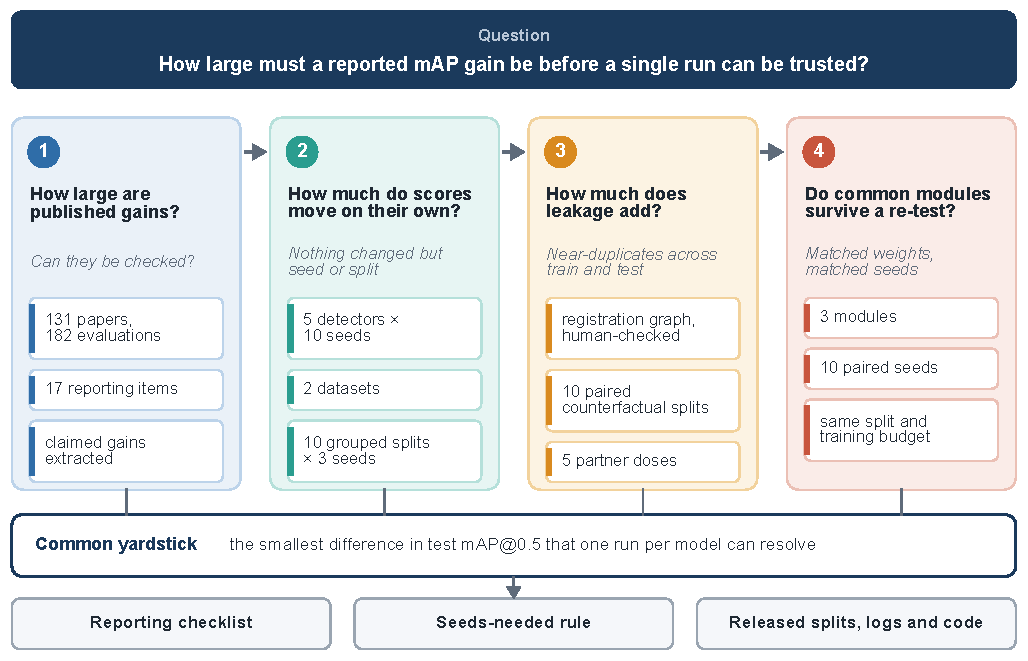
\includegraphics[width=\textwidth]{figures/figA_framework.pdf}
\caption{The four questions of this study and the yardstick shared by all of them.}
\label{fig:framework}
\end{figure*}

The answers do not line up with the usual suspicion that leakage is the main problem. Leakage is real: on the test images that have a duplicate in training, mAP@0.5 rises by 4.1 points. But those images are about one sixth of a randomly split test set, and the score of the whole test set moves by 0.4 points, which is not distinguishable from zero. Seed noise is several times larger. With one run per model, a gain has to exceed 2.2--3.5 points on NEU-DET and 4.0--5.5 points on GC10-DET before it can be told apart from chance, and about 8 points if the two models were trained on different splits. \todo{State what share of published gains falls below these thresholds once the extraction table has been cleaned.} Almost no paper reports the seeds, splits or repeated runs that a reader would need to check.

The contributions are therefore: (i) an audit of what the NEU-DET and GC10-DET detection literature reports, with the claimed gains; (ii) a measured resolution limit for single-run comparisons on both datasets, and a rule for the number of seeds a claim of a given size needs; (iii) a hand-checked graph of overlapping images in NEU-DET, grouped splits derived from it, and a paired estimate of what leakage adds; and (iv) released splits, run logs and code. Section~\ref{sec:related} places the work, Sections~\ref{sec:lit_method}--\ref{sec:lit_results} report the audit, Sections~\ref{sec:bench_design}--\ref{sec:bench_results} the experiments, and Section~\ref{sec:discussion} what follows for practice.

\section{Related Work}\label{sec:related}

\subsection{Public Benchmarks and Architectural Proliferation in Steel Defect Detection}
Since its introduction by \citet{song2013neu} and expansion to bounding-box annotations by \citet{he2020neu}, NEU-DET (1,800 grayscale $200\times 200$ hot-rolled strip images across six classes: \textit{crazing}, \textit{inclusion}, \textit{patches}, \textit{pitted surface}, \textit{rolled-in scale}, and \textit{scratches}) has served as the primary public testbed for flat-steel inspection. \citet{lv2020gc10} subsequently introduced GC10-DET, comprising high-resolution cold-rolled strip images across ten defect categories. Recent surveys chronicle an explosion of neural architectures tailored to these two datasets \citep{cheng2026survey}, overwhelmingly built on single-stage YOLO backbones \citep{chen2022_pmc8838028,nguyen2022_pmc9783860,zhang2023_pmc10582940,wang2025_pmc12491516,rong2026_pmc13708875,li2026dpsnet} augmented with channel-spatial attention modules \citep{woo2018cbam,ouyang2023ema,duan2026_pmc12881659,sun2026_pmc13412141}, frequency-domain or wavelet branches \citep{sun2025_pmc12298282,ge2026_pmc13004511,chen2026_pmc13562717,wei2026amfnet,liu2025sfc}, state-space Mamba blocks \citep{jin2026_pmc13280455}, or bidirectional feature fusion necks \citep{tan2020efficientdet,zhou2026_pmc13030490,xing2026_pmc13194957}. Despite this intense modeling activity, neither NEU-DET nor GC10-DET shipped an official train/validation/test split manifest, leaving nearly every paper to construct an undisclosed private random split (e.g., 7:2:1, 8:1:1, or 8:2) \citep{lema2025reproducible}.

\subsection{Protocol Sensitivity, Stochastic Variance, and Reporting Standards}
Across empirical machine learning, unstandardized evaluation pipelines and single-seed point estimates frequently obscure true model progress \citep{gundersen2018state,dodge2019show,musgrave2020reality,pineau2021improving}. \citet{picard2021torch} and \citet{bouthillier2021accounting} demonstrated that varying random seeds or partition realizations can shift vision accuracy by 1--3 pp, overlapping many incremental claims. In object detection specifically, \citet{ghahremani2026initialization} showed that weight initialization transfer, epoch budget, and detector architecture interact strongly, and that apparent gains often vanish when baselines are retrained under strictly matched initialization and budgets. While general frameworks such as REFORMS \citep{kapoor2024reforms} and Datasheets for Datasets \citep{gebru2021datasheets} establish reporting principles, no prior study has audited quantitative protocol compliance across the peer-reviewed steel-defect detection corpus or directly calibrated claimed $\Delta\text{mAP@0.5}$ distributions against multi-split variance, multi-seed noise, and counterfactual duplicate leakage.

\subsection{Near-Duplicate Leakage and Comparison with Adjacent Work}
Train--test contamination via exact copies (\textit{hard leakage}) or overlapping crops and adjacent sequence frames (\textit{soft leakage}) is known to inflate metrics across natural images \citep{barz2020cifair,recht2019imagenet,ramos2025leakage} and medical imaging \citep{tampu2022inflation,roberts2021common,varoquaux2022evaluating}. In continuous strip rolling, linescan cameras acquire consecutive frames along a coil pass \citep{technologies2026review,molleda2026edge}; when shifted or rotated patches cropped from the same physical defect scene straddle train and test splits, detectors can exploit shared background scale texture and defect geometry. To delineate our scope transparently against the closest prior and concurrent studies, Table~\ref{tab:adjacent_work} summarizes methodological differences item by item.

\begin{table}[htbp]
\centering
\footnotesize
\setlength{\tabcolsep}{3pt}
\caption{Structured comparison with closest prior and concurrent studies on steel-defect protocol reproducibility and near-duplicate data leakage.}
\label{tab:adjacent_work}
\begin{tabularx}{\textwidth}{>{\raggedright\arraybackslash}p{2.3cm} >{\raggedright\arraybackslash}p{3.0cm} >{\raggedright\arraybackslash}p{3.1cm} >{\raggedright\arraybackslash}X}
\toprule
\textbf{Study} & \textbf{Scope \& Data} & \textbf{Audit / Deduplication} & \textbf{Distinction of Present Work} \\
\midrule
\citet{lema2025reproducible} & 18 YOLO models on 4-fold stratified NEU-DET CV & Parametric/non-parametric fold ranking tests & Adds 131-paper 17-field audit, $\mathrm{SE}(2)$ registration grouping so duplicate rolling components never straddle folds, and paired counterfactual leakage estimates. \\
\citet{technologies2026review} & Qualitative review of steel inspection evaluation pitfalls & Conceptual slice- vs.\ sequence-leakage taxonomy & Operationalizes the taxonomy into a 17-field verbatim corpus audit (182 evaluations) and an algorithmic registration pipeline when coil IDs are absent. \\
\citet{molleda2026edge} & Proprietary 3,097-image instance-segmentation line dataset & pHash + timestamps; discards 139 of 285 test images & Public NEU-DET lacks timestamps and has $90^\circ$-rotated partial crops (60\%+ overlap); MIP grouping yields no registration-detected cross-split pair without deleting test samples. \\
\citet{bourezgui2026rock} & Geological rock image classification benchmarks & SIFT/RANSAC grouping + observational subset splits & Multi-object $\text{mAP}$ is confounded by class/scale differences in naive subsets; uses $K=10$ matched counterfactual partner swaps plus fixed-FP escape rates. \\
\citet{chen2026confidence,yang2026improved} & Dataset cleaning notes within detector papers & Hash duplicate pair (NEU-DET) / 12 dups removed (GC10) & Both recorded as positive audit items; full 223-edge $\mathrm{SE}(2)$ graph and 467-coil GC10 partitioning systematically resolve hidden overlaps. \\
\citet{jeong2026zenodo,li2026figshare} & Concurrent data archives on NEU-DET / GC10-DET & Image splits / GC10 prefix \& thumbnail checks & Provides full 17-field verbatim audit, human-verified $\mathrm{SE}(2)$ NEU graph, component-disjoint MIP splits, and counterfactual dose curves. \\
\bottomrule
\end{tabularx}
\end{table}

\section{Systematic Literature Audit Methodology}\label{sec:lit_method}

\subsection{Search Strategy, Corpus Boundary, and Eligibility Criteria}
{\emergencystretch=3em
Following PRISMA 2020 guidelines \citep{page2021prisma}, we executed three programmatic queries on the Europe PMC REST API on October 30, 2026 covering publications from January 1, 2020 to October 30, 2026 (\texttt{FIRST\_PDATE:[2020-01-01 TO 2026-10-30]}): (q1) \texttt{TITLE\_ABS:(steel AND defect AND yolo*)}, (q2) \texttt{TITLE\_ABS:(steel AND defect AND (detect* OR inspection))}, and (q3) \texttt{(TITLE\_ABS:"NEU-DET" OR TITLE\_ABS:"GC10-DET")}. Union deduplication by normalized DOI (or source identifier when DOI was absent) yielded 433 unique candidate records. Europe PMC indexes the PubMed Central (PMC) full-text open-access journal archive alongside MEDLINE metadata and external preprint records. Because closed-access subscription articles without PMC deposit and standalone external preprints are not distributed as PMC JATS XML, full-text extraction evaluates the peer-reviewed PMC open-access journal cohort while accounting explicitly for every one of the 61 non-XML records (Table~\ref{tab:prisma} and Figure~\ref{fig:prisma_flow}). In addition, a prospective cross-database sampling protocol covering Scopus and Web of Science Core Collection for non-PMC journal articles is documented in our companion repository.\par}

\begin{figure*}[t]
\centering
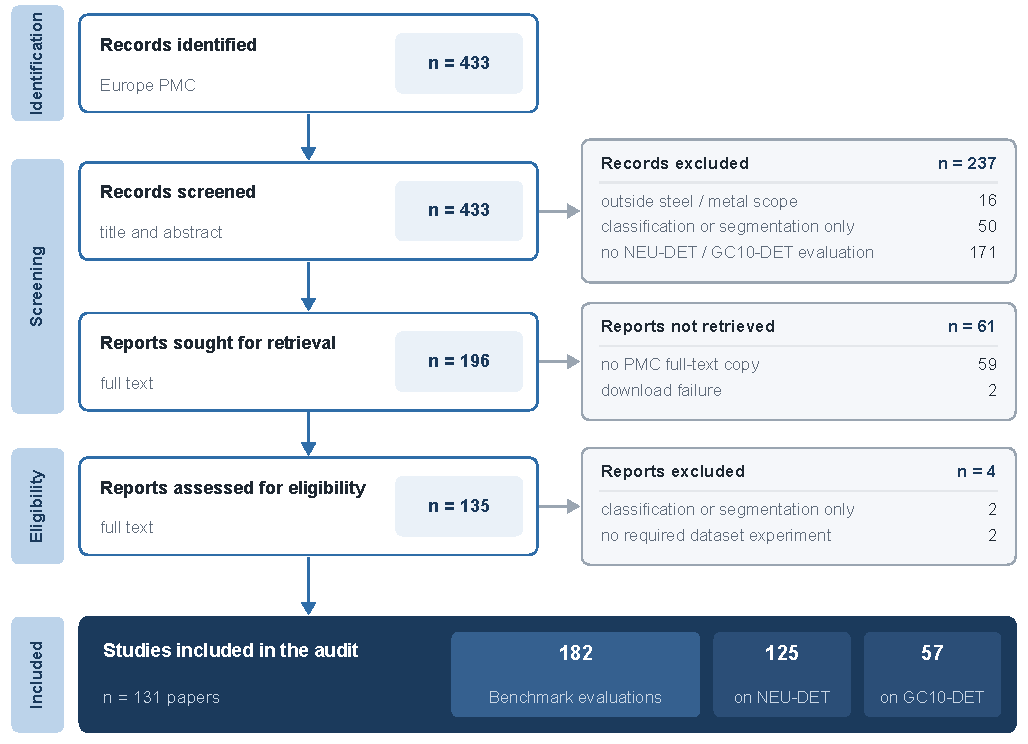
\includegraphics[width=\textwidth]{figures/fig02_prisma.pdf}
\caption{PRISMA 2020 flow diagram documenting record identification ($N=433$), title and abstract screening ($N=237$ excluded, $N=196$ retained), programmatic PMC JATS XML retrieval ($N=135$ retrieved, $N=61$ non-XML records itemized across E4 duplicate/superseded versions and E5 unretrieved non-XML records), full-text eligibility assessment ($N=4$ excluded), and final inclusion ($N=131$ peer-reviewed PMC journal articles, 0 preprints; $182$ benchmark evaluations).}
\label{fig:prisma_flow}
\end{figure*}

We applied pre-specified eligibility rules during screening and full-text assessment:
\begin{itemize}[leftmargin=2em, itemsep=0.1em]
    \item \textbf{Inclusion Criteria}: English-language original peer-reviewed research articles (2020--October 30, 2026) with accessible full text reporting quantitative bounding-box object detection experiments on NEU-DET or GC10-DET.
    \item \textbf{Exclusion Codes}: \texttt{E1}, non-original research (reviews, editorials); \texttt{E2}, classification or pixel segmentation only without bounding-box detection; \texttt{E3}, no evaluation on NEU-DET or GC10-DET; \texttt{E4}, duplicate record or preprint superseded by a formal journal article; \texttt{E5}, programmatic full-text JATS XML unavailable; \texttt{E6}, non-English publication.
\end{itemize}

\subsection{Protocol Coding Schema (F01--F17) and Claimed Delta Extraction}
Each of the 182 dataset evaluations (125 on NEU-DET, 57 on GC10-DET) across the 131 included studies was coded across 17 discrete protocol dimensions (\texttt{F01}--\texttt{F17}) spanning the object detection pipeline (Figure~\ref{fig:pipeline_f01_f17}):
\begin{enumerate}[leftmargin=2em, itemsep=0.05em]
    \item \textbf{Dataset \& Split Hygiene}: \texttt{F01} Dataset version/source link; \texttt{F02} Nominal split ratio or image counts; \texttt{F03} Reconstructible split manifest (file list or deterministic script); \texttt{F04} Near-duplicate or identity leakage audit disclosure.
    \item \textbf{Training Configuration}: \texttt{F05} Pretraining weight source (scratch vs.\ COCO/ImageNet pretrained); \texttt{F09} Training and testing input dimensions ($W \times H$); \texttt{F10} Epoch or iteration budget; \texttt{F11} Batch size.
    \item \textbf{Evaluation Isolation \& Checkpoint Selection}: \texttt{F06} Checkpoint selection rule (best validation fitness vs.\ last epoch); \texttt{F07} Evaluation split naming clarity (distinguishing validation vs.\ test); \texttt{F08} Physical separation between validation tuning set and held-out test set.
    \item \textbf{Stochastic Uncertainty \& Baseline Provenance}: \texttt{F12} Random seed disclosure; \texttt{F13} Multiple runs with dispersion (SD, SE, or CI); \texttt{F14} Baseline retraining provenance (retrained under matched protocol vs.\ copied from literature).
    \item \textbf{Deployment \& Open Artifacts}: \texttt{F15} Inference hardware, batch size, and latency scope; \texttt{F16} Open-source code repository link; \texttt{F17} Publicly downloadable trained model weights.
\end{enumerate}

\begin{figure*}[t]
\centering
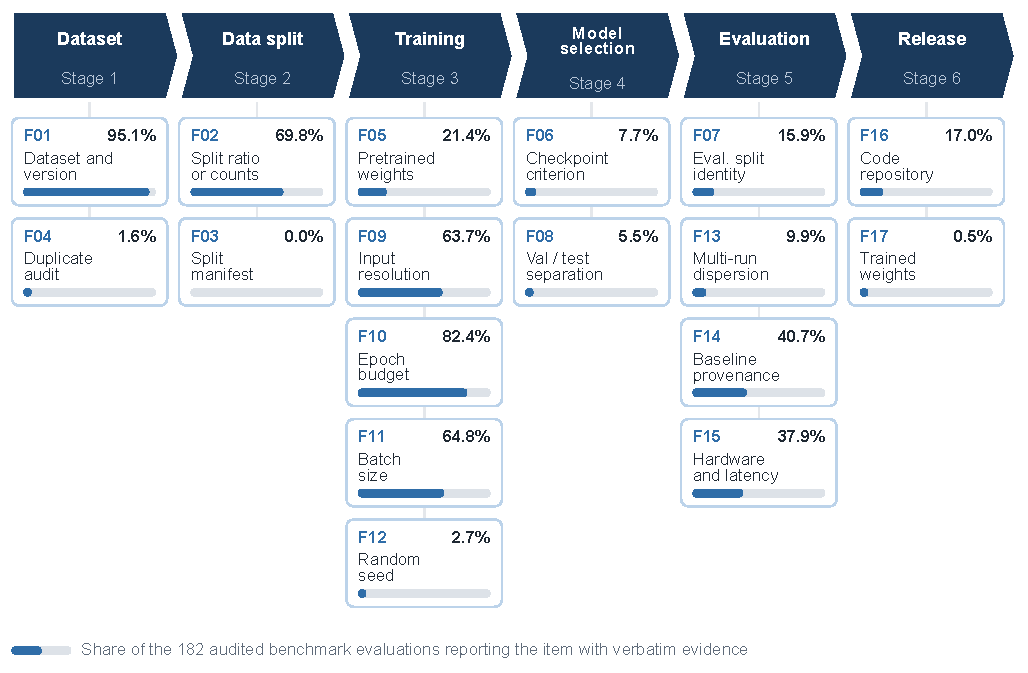
\includegraphics[width=\textwidth]{figures/fig03_protocol_pipeline.pdf}
\caption{End-to-end object detection benchmark pipeline mapping the 17 audited protocol dimensions (F01--F17) across data curation, splitting, training initialization, checkpoint selection, held-out testing, and artifact release, alongside audited positive reporting rates across 182 evaluations.}
\label{fig:pipeline_f01_f17}
\end{figure*}

Every field was classified as \texttt{reported}, \texttt{ambiguous}, or \texttt{not\_reported\_in\_paper}. Positive (\texttt{reported}) or \texttt{ambiguous} decisions required an exact verbatim quotation ($\le 35$ words) verified by automated substring matching against the publisher JATS XML, paired with Wilson score 95\% confidence intervals \citep{wilson1927probable}. Additionally, we parsed all JATS XML tables and results sections across the 182 evaluations to extract verbatim baseline $\text{mAP@0.5}$, proposed model $\text{mAP@0.5}$, and claimed improvement $\Delta\text{mAP@0.5} = \text{mAP}_{\text{proposed}} - \text{mAP}_{\text{baseline}}$.

\paragraph{Who coded what.} A large language model (\todo{name and version}) produced the first-pass code and the supporting quotation for every field. \todo{Complete before submission and then rewrite this sentence in the past tense: two authors independently re-code the six fields on which our conclusions rest (\texttt{F03}, \texttt{F04}, \texttt{F07}, \texttt{F08}, \texttt{F12}, \texttt{F13}) for all 182 evaluations without seeing the model output, and resolve disagreements by discussion; report Cohen's $\kappa$ and Gwet's AC1 per field.} The remaining eleven fields were checked by one author against the quotation. Claimed gains were extracted by script from the results tables and then \todo{checked by hand against each paper; define the baseline as the model named as baseline in the paper's own ablation table, and drop evaluations without one}. All rates below use the human-adjudicated codes.

\section{Systematic Literature Audit Findings}\label{sec:lit_results}

\subsection{PRISMA Disposition and Audit Reliability}
Table~\ref{tab:prisma} itemizes all 433 screened records and accounts for all 61 non-XML records: 8 duplicate or superseded versions (\texttt{E4}, including 5 whose formal journal versions are inside our 131-paper corpus), 37 standalone preprints without PMC XML (\texttt{E5}), 2 PMC server HTTP 500 errors (\texttt{E5}), and 14 MEDLINE-only records lacking open-access links (\texttt{E5}). Among 135 full-text XML articles assessed, 4 were excluded (2 classification/segmentation only [\texttt{E2}], 2 lacking NEU/GC10 detection [\texttt{E3}]), leaving 131 peer-reviewed journal articles (182 evaluations).

\begin{table}[htbp]
\centering
\footnotesize
\setlength{\tabcolsep}{3.5pt}
\caption{PRISMA 2020 selection, retrieval, and non-XML disposition ledger for the Europe PMC screening corpus ($N=433$).}
\label{tab:prisma}
\begin{tabularx}{\textwidth}{>{\raggedright\arraybackslash}p{2.3cm} r X}
\toprule
\textbf{Stage} & \textbf{Count} & \textbf{Recorded evidence and disposition} \\
\midrule
Identification & 433 & Unique records from 3 Europe PMC queries (\texttt{2020-01-01} to \texttt{2026-10-30}), deduplicated by DOI/source ID. \\
Screening & 433 & 237 exclusions: 16 outside steel/metal scope, 50 classification/segmentation only, 171 without NEU/GC10 evaluation. \\
Retained for retrieval & 196 & 154 \texttt{include\_ft} and 42 \texttt{unclear\_ft} decisions (137 with initial PMCIDs, 59 without). \\
PMC XML retrieval & 137 & 135 successful JATS XML downloads and 2 HTTP 500 server failures (\texttt{PMC13074744}, \texttt{PMC13492231}). \\
Outside XML set & 61 & \textbf{47 with OA metadata links}: 8 duplicate/superseded records (\texttt{E4}: 2 duplicate MEDLINE entries and 3 preprints of articles already in the 131 included studies, plus 3 preprints superseded by other journal versions); 37 standalone external preprints without PMC JATS XML (\texttt{E5}); 2 PMC HTTP 500 failures (\texttt{E5}). \textbf{14 without OA links}: 14 MEDLINE-only journal records lacking PMCIDs and OA links (\texttt{E5}). \\
Full-text assessment & 135 & 4 exclusions (2 classification/segmentation only [\texttt{E2}]; 2 without NEU-DET/GC10-DET experiments [\texttt{E3}]). \\
Included corpus & 131 & 131 peer-reviewed PMC journal articles (0 preprints), covering 182 benchmark evaluations (125 NEU-DET, 57 GC10-DET) with 1,266 verbatim-verified evidence quotations. \\
\bottomrule
\end{tabularx}
\end{table}

\paragraph{How reliable is the coding?} \todo{Replace this paragraph with the human inter-coder agreement once dual coding is complete.} The only agreement figures available at present compare two model-assisted coding passes on a 26-paper sample (35 evaluations, 595 ratings): raw agreement 83.5\%, Cohen's $\kappa=0.722$ \citep{cohen1960coefficient}, Gwet's $\text{AC1}=0.791$ \citep{gwet2008computing}. They describe the consistency of the extraction pipeline and are not evidence of human reliability. Agreement was high for items that are stated as numbers (\texttt{F01}, \texttt{F02}, \texttt{F09}--\texttt{F11}; $\text{AC1}>0.90$) and low for the three items that require interpretation (\texttt{F07}, \texttt{F08}, \texttt{F14}; $\kappa=0.319$, $0.099$, $0.128$). The rates for those three items should be read as provisional until they have been coded by hand.

\subsection{Reporting Completeness Across 17 Protocol Dimensions}
Figure~\ref{fig:reporting_completeness} and Table~\ref{tab:audit_table} summarize compliance across all 182 evaluations:
\begin{enumerate}[leftmargin=2em]
    \item \textbf{Absence of Split Manifests (\texttt{F03}) and Duplicate Screening (\texttt{F04})}: While 69.8\% (127/182; 95\% Wilson CI $[62.8\%, 76.0\%]$) state a nominal split ratio such as 8:1:1 or 7:2:1 (\texttt{F02}), \textbf{0.0\%} (0/182; 95\% CI $[0.0\%, 2.1\%]$) release a reconstructible split manifest (\texttt{F03}). Only \textbf{1.6\%} (3/182; 95\% CI $[0.6\%, 4.7\%]$) mention any duplicate screening (\texttt{F04}): \citet{chen2026confidence} on NEU-DET and \citet{yang2026improved} on NEU-DET and GC10-DET.
    \item \textbf{Omission of Random Seeds (\texttt{F12}) and Multi-Run Dispersion (\texttt{F13})}: Only \textbf{2.7\%} (5/182; e.g., \citealp{hu2026_pmc12986859,zhu2026_pmc13418091,huang2026_pmc13618933}) disclose random seeds, and \textbf{89.0\%} (162/182) report single-point scores without SD, SE, or CI (\texttt{F13} reported in 18/182 or \textbf{9.9\%}, e.g., \citealp{zhang2025_pmc12350654,fan2025_pmc12770479,duan2026_pmc12881659,wang2026_pmc13029871,zhang2026_pmc13056895,jin2026_pmc13280455,sun2026_pmc13412141,rong2026_pmc13708875}).
    \item \textbf{Validation--Test Conflation (\texttt{F07}, \texttt{F08}) and Artifact Scarcity (\texttt{F16}, \texttt{F17})}: Only \textbf{15.9\%} (29/182) clearly distinguish validation vs.\ test evaluation splits (\texttt{F07}, e.g., \citealp{wang2023_pmc10300763,zhang2023_pmc10582940,ma2023_pmc10675464,chen2023_pmc10719359,zou2024_pmc10935385,gao2024_pmc11001973,wang2024_pmc11091066,sun2025_pmc12298282}), and just \textbf{5.5\%} (10/182, e.g., \citealp{chen2022_pmc8838028,nguyen2022_pmc9783860,ma2023_pmc10675464,zou2024_pmc10935385,ahangar2026_pmc12899597,chen2026_pmc13562717,huang2026_pmc13618933,yang2026improved}) document physical separation between validation checkpoint selection and held-out testing (\texttt{F08}). Only 17.0\% (31/182) share code URLs (\texttt{F16}) and 0.5\% (1/182) release weights (\texttt{F17}). Across all 17 items, an evaluation reports on average $5.37 \pm 2.07$ of 17 items (median $5.0$, IQR $[4.0, 6.0]$).
    \item \textbf{Claimed gains.} \todo{Rewrite from the cleaned table. The current extraction gives a median near 3.8~pp with an interquartile range of about 2--7~pp, but it mixes baselines of different kinds (a paper's own base model in some rows, an unrelated comparison detector in others) and contains mis-parsed table rows. Two extractions disagree and neither is final: \texttt{results/step4\_claimed\_deltas\_182.json} ($n=174$, median 3.80~pp) and \texttt{docs/coding\_v1/rollup\_20261103.json} ($n=177$, median 2.5~pp); figD currently plots the former. Report $n$, median and interquartile range for the cleaned set, separately for NEU-DET and GC10-DET.}
\end{enumerate}

\begin{figure*}[t]
\centering
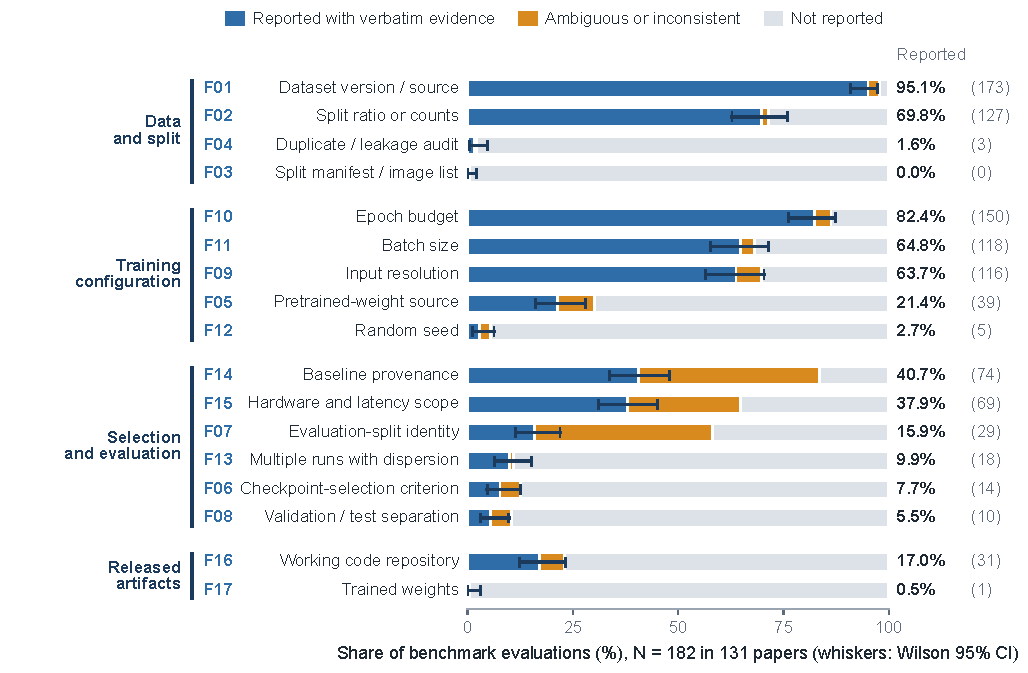
\includegraphics[width=\textwidth]{figures/fig04_reporting_completeness.pdf}
\caption{Protocol reporting completeness across 17 pre-specified dimensions (F01--F17) for 182 benchmark evaluations in 131 peer-reviewed PMC articles, grouped by methodological stage with horizontal 95\% Wilson confidence intervals on positive reporting rates.}
\label{fig:reporting_completeness}
\end{figure*}

\begin{table}[htbp]
\centering
\footnotesize
\setlength{\tabcolsep}{2.5pt}
\caption{Reporting completeness across 17 protocol dimensions for 182 evaluated benchmark experiments on NEU-DET ($n=125$) and GC10-DET ($n=57$) across 131 included articles, with 95\% Wilson CIs. $^{\dagger}$F04 reflects the verified count including \citet{chen2026confidence} and \citet{yang2026improved}.}
\label{tab:audit_table}
\begin{tabularx}{\textwidth}{l >{\raggedright\arraybackslash}X r r r r}
\toprule
\textbf{ID} & \textbf{Protocol Dimension} & \textbf{Reported} & \textbf{95\% Wilson CI} & \textbf{Ambiguous} & \textbf{Not Rep.} \\
\midrule
\textbf{F01} & Dataset Version / Source Link & 173 (95.1\%) & [90.9\%, 97.4\%] & 5 (2.7\%) & 4 (2.2\%) \\
\textbf{F02} & Split Ratio / Sample Counts & 127 (69.8\%) & [62.8\%, 76.0\%] & 3 (1.6\%) & 52 (28.6\%) \\
\textbf{F03} & Split Manifest / Image List Link & \textbf{0 (0.0\%)} & [0.0\%, 2.1\%] & 1 (0.5\%) & \textbf{181 (99.5\%)} \\
\textbf{F04} & Duplicate Leakage Audit$^{\dagger}$ & \textbf{3 (1.6\%)} & [0.6\%, 4.7\%] & 1 (0.5\%) & \textbf{178 (97.8\%)} \\
\textbf{F05} & Pretraining Weight Source & 39 (21.4\%) & [16.1\%, 27.9\%] & 16 (8.8\%) & 127 (69.8\%) \\
\textbf{F06} & Checkpoint Selection Metric & 14 (7.7\%) & [4.6\%, 12.5\%] & 9 (4.9\%) & 159 (87.4\%) \\
\textbf{F07} & Eval.\ Set Clarity (Val vs.\ Test) & 29 (15.9\%) & [11.3\%, 21.9\%] & 77 (42.3\%) & 76 (41.8\%) \\
\textbf{F08} & Validation vs.\ Test Separation & \textbf{10 (5.5\%)} & [3.0\%, 9.8\%] & 9 (4.9\%) & 163 (89.6\%) \\
\textbf{F09} & Train \& Test Input Dimensions & 116 (63.7\%) & [56.5\%, 70.4\%] & 11 (6.0\%) & 55 (30.2\%) \\
\textbf{F10} & Epoch Budget & 150 (82.4\%) & [76.2\%, 87.3\%] & 7 (3.8\%) & 25 (13.7\%) \\
\textbf{F11} & Batch Size & 118 (64.8\%) & [57.7\%, 71.4\%] & 6 (3.3\%) & 58 (31.9\%) \\
\textbf{F12} & Explicit Random Seed & \textbf{5 (2.7\%)} & [1.2\%, 6.3\%] & 5 (2.7\%) & \textbf{172 (94.5\%)} \\
\textbf{F13} & Multiple Runs with Dispersion & \textbf{18 (9.9\%)} & [6.3\%, 15.1\%] & 2 (1.1\%) & \textbf{162 (89.0\%)} \\
\textbf{F14} & Baseline Provenance & 74 (40.7\%) & [33.8\%, 47.9\%] & 78 (42.9\%) & 30 (16.5\%) \\
\textbf{F15} & Inference Hardware \& Scope & 69 (37.9\%) & [31.2\%, 45.1\%] & 49 (26.9\%) & 64 (35.2\%) \\
\textbf{F16} & Open-Source Code Link & 31 (17.0\%) & [12.3\%, 23.2\%] & 11 (6.0\%) & 140 (76.9\%) \\
\textbf{F17} & Trained Weights Accessibility & \textbf{1 (0.5\%)} & [0.1\%, 3.0\%] & 0 (0.0\%) & \textbf{181 (99.5\%)} \\
\bottomrule
\end{tabularx}
\end{table}

\section{Benchmark Design: Finding Overlapping Images and Building Grouped Splits}\label{sec:bench_design}

\subsection{Registration Graph and Grouped Partitions}\label{sec:frozen_partition}
To prevent overlapping or consecutive strip patches from straddling training and evaluation sets when acquisition timestamps are unavailable, we developed a three-stage $\mathrm{SE}(2)$ registration and graph-partitioning pipeline (Figure~\ref{fig:reg_pipeline}):
\begin{enumerate}[leftmargin=2em]
    \item \textbf{Stage 1 (Coarse Screening) and Stage 2 (Subpixel Phase Refinement)}: Across all $1,613,706$ unordered pairs among 1,797 valid NEU-DET images, images are downsampled to $16 \times 16$ via area interpolation and screened over translations $|\Delta x|, |\Delta y| \le 0.25 W$ ($\pm 50\text{ px}$ at $200\times 200$) with minimum overlap fraction $\ge 0.60$ across four discrete quarter-turn rotations ($k\in\{0^\circ, 90^\circ, 180^\circ, 270^\circ\}$) via Fast Fourier Transform (FFT) normalized cross-correlation \citep{lewis1995fast}. Pairs clearing the coarse gate ($\text{NCC}_{\text{coarse}} \ge 0.85$; $122,706$ pairs) plus a marginal audit band ($\text{NCC}_{\text{coarse}} \in [0.80, 0.85)$; $96,572$ pairs) undergo $64\times 64$ phase-correlation subpixel refinement \citep{foroosh2002extension} and native $200\times 200$ integer-offset verification.
    \item \textbf{Stage 3 (Native Dual Pixel/Gradient NCC Verification)}: Over the overlapping region $\Omega$ ($\text{area}(\Omega) \ge 0.60$), we enforce joint pixel-intensity $I$ and $3\times 3$ Sobel gradient $G = (\partial_x I, \partial_y I)$ thresholds:
    \begin{align}
        \text{NCC}_{\text{pixel}}(I_A, I_B) &= \frac{\sum_{\Omega} (I_A - \mu_A)(I_B - \mu_B)}{\sqrt{\sum_{\Omega} (I_A - \mu_A)^2 \sum_{\Omega} (I_B - \mu_B)^2}} \ge 0.95, \\
        \text{NCC}_{\text{grad}}(G_A, G_B) &= \frac{\sum_{\Omega} (G_A - \bar{G}_A) \cdot (G_B - \bar{G}_B)}{\|G_A - \bar{G}_A\|_2 \|G_B - \bar{G}_B\|_2} \ge 0.90.
    \end{align}
    Threshold design reflects complementary physical constraints: $\text{NCC}_{\text{pixel}} \ge 0.95$ tolerates minor JPEG compression artifacts ($\text{MAE}$ up to $\sim 2.5\text{ ADU}/255$ on compressed crops) while rejecting coincidental background brightness similarities, whereas $\text{NCC}_{\text{grad}} \ge 0.90$ enforces fine structural scratch/scale edge congruence so smooth illumination patches cannot pass as false positives. The primary pass yields 219 verified edges and the $[0.80, 0.85)$ coarse band captures 4 additional edges (all with native $\text{NCC}_{\text{pixel}} \ge 0.9884$ and $\text{NCC}_{\text{grad}} \ge 0.9849$), totaling \textbf{223 near-duplicate edges} (native $\text{NCC}_{\text{pixel}} \in [0.9520, 1.0000]$, median $0.9955$; $\text{NCC}_{\text{grad}} \in [0.9025, 1.0000]$, median $0.9884$; overlap $\in [0.6006, 0.9700]$). Figure~\ref{fig:reg_examples} verifies this mechanism directly at native pixels: \texttt{scratches\_254} vs.\ \texttt{scratches\_249} align under a $0^\circ$ crop translation $(\Delta x,\Delta y)=(-40, +40)\text{ px}$ sharing $64.0\%$ of the $200\times 200$ canvas with $\text{NCC}_{\text{pixel}}=1.0000$ and zero pixel residual ($\text{MAE}=0.000\text{ ADU}/255$), while \texttt{scratches\_157} vs.\ \texttt{scratches\_279} undergo a $90^\circ$ rotation plus $(0,-40)\text{ px}$ shift over $80.0\%$ overlap ($\text{NCC}_{\text{pixel}}=0.9990$, $\text{MAE}=0.814\text{ ADU}/255$).
\end{enumerate}

\begin{figure*}[t]
\centering
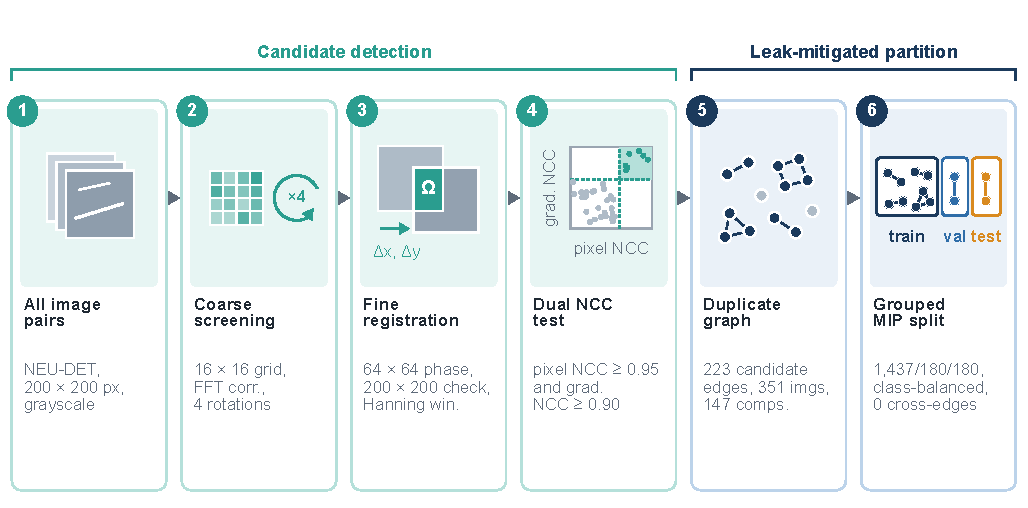
\includegraphics[width=\textwidth]{figures/fig05_duplicate_pipeline.pdf}
\caption{Multi-stage $\mathrm{SE}(2)$ registration and mixed-integer programming (MIP) partition pipeline. Candidate pairs pass through $16\times 16$ FFT coarse screening across four quarter-turn rotations, $64\times 64$ phase-correlation subpixel refinement with native $200\times 200$ verification, and dual pixel/gradient NCC thresholding ($\text{NCC}_{\text{pixel}}\ge 0.95 \land \text{NCC}_{\text{grad}}\ge 0.90$, overlap $\ge 0.60$), yielding 147 connected components assigned intact to train/val/test partitions (80/10/10) with zero cross-split edges.}
\label{fig:reg_pipeline}
\end{figure*}

\begin{figure*}[t]
\centering
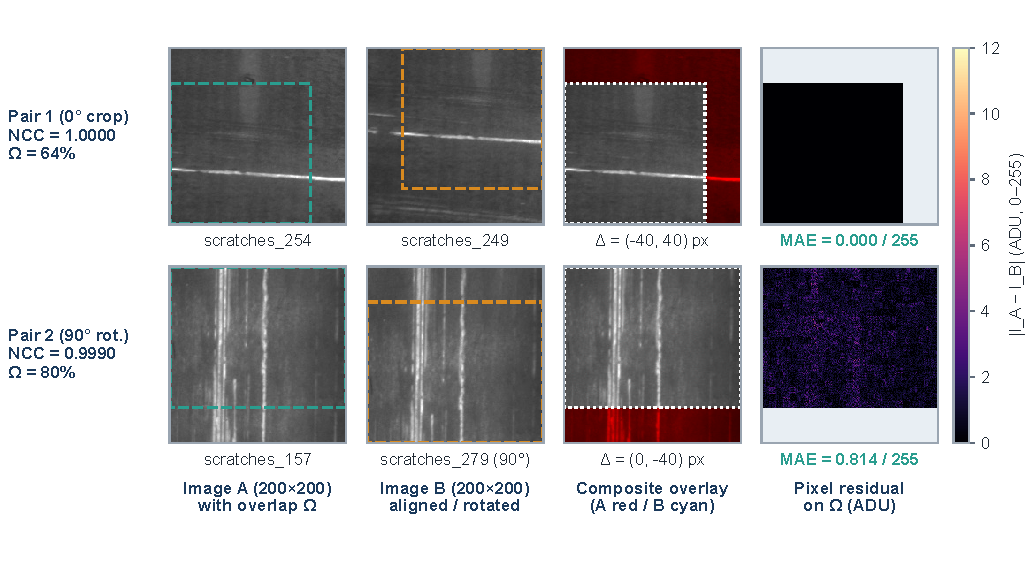
\includegraphics[width=\textwidth]{figures/fig06b_registration_examples.pdf}
\caption{Pixel-level $\mathrm{SE}(2)$ registration verification on representative NEU-DET near-duplicate pairs. Top row: translation-crop pair (\texttt{scratches\_254} vs.\ \texttt{scratches\_249}, $0^\circ$, $\Delta=(-40,+40)\text{ px}$, $64\%$ overlap, $\text{NCC}_{\text{pixel}}=1.0000$) exhibits exact zero pixel residual ($\text{MAE}=0.000\text{ ADU}/255$) inside $\Omega$. Bottom row: $90^\circ$-rotated and shifted pair (\texttt{scratches\_157} vs.\ \texttt{scratches\_279}, $\Delta=(0,-40)\text{ px}$, $80\%$ overlap, $\text{NCC}_{\text{pixel}}=0.9990$) aligns to $\text{MAE}=0.814\text{ ADU}/255$. False-color composites render Image A in red and registered Image B in cyan (neutral gray indicates agreement inside $\Omega$).}
\label{fig:reg_examples}
\end{figure*}

\begin{figure*}[t]
\centering
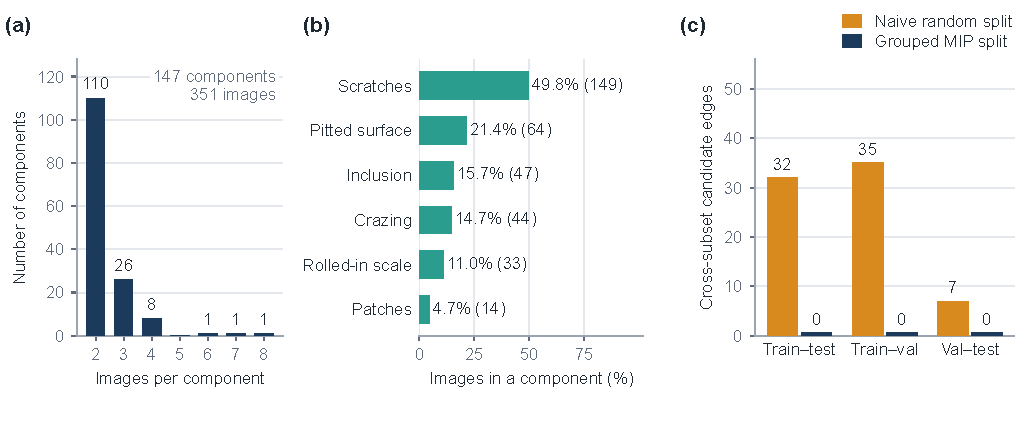
\includegraphics[width=\textwidth]{figures/fig06_duplicate_statistics.pdf}
\caption{Near-duplicate graph topology and cross-split leakage statistics across NEU-DET ($N=1,797$). (a) Connected-component size distribution across the 147 multi-image components (351 images, 100\% class-prefix purity). (b) Per-category share of images in multi-image near-duplicate components. (c) Cross-split near-duplicate edges under naive stratified random splitting (74 cross-split edges: 32 train--test, 35 train--val, 7 val--test) versus MIP grouped partitioning (0 cross-split edges).}
\label{fig:ncc_components}
\end{figure*}

\begin{itemize}[leftmargin=2em]
    \item \textbf{Pre-MIP Deduplication, Graph Topology, and MIP Partitions}: Before connected-component grouping, three near/exact duplicate images from three isolated 2-image pairs in the raw 1,800-image release were removed during pairwise deduplication: \texttt{patches\_105} (paired with \texttt{patches\_101}, matching the content-hash pair noted by \citealp{chen2026confidence}), \texttt{pitted\_surface\_292} (paired with \texttt{pitted\_surface\_171}), and \texttt{scratches\_247} (paired with \texttt{scratches\_232}), leaving each remaining image as a clean singleton. All remaining 223 pairs were retained intact and grouped as connected components to preserve full sample size ($N=1,797$) and class balance. Across the 1,797 images, these 223 edges span 351 images (19.5\%) and form \textbf{147 multi-image components} (110 pairs, 26 triplets, 8 quadruplets, and larger clusters of 6, 7, and 8 frames; 100\% class-prefix purity; Figure~\ref{fig:ncc_components}a--b). Threshold sensitivity analysis (Table~\ref{tab:threshold_sensitivity}) confirms strong structural stability even when native criteria are tightened to $\text{NCC}_{\text{pixel}}\ge 0.99 \land \text{NCC}_{\text{grad}}\ge 0.98$ (retaining 134 edges across 219 images). Using mixed-integer linear programming (MIP), all 147 components and 1,446 singletons are allocated into exact class-balanced 80.0\%/10.0\%/10.0\% partitions (1,437 train / 180 val / 180 test) with \textbf{zero cross-split edges}. We establish an initial pilot grouped split (\textbf{NEU-Pilot}) alongside our primary, freshly drawn independent grouped benchmark (\textbf{NEU-Grouped}, having 0/180 validation or test overlap with \textbf{NEU-Pilot}) and a filename-group-disjoint MIP partition on GC10-DET (\textbf{GC10-CoilGrouped}, 1,831 train / 230 val / 230 test across 467 filename groups, 0 cross-split coil edges).
    \item \textbf{Checking the graph by hand.} The two authors independently inspected 349 candidate pairs without seeing each other's labels or the registration scores: all 223 graph edges, 26 pairs that fell just below the registration thresholds, and 100 pairs proposed by ResNet-50 feature similarity or ORB matching (Figure~\ref{fig:dup_evidence}c). Of the 223 edges, both annotators confirmed 184 (82.5\%), one confirmed a further 36, and both rejected 3; agreement on the edges was 83.9\% (Gwet's $\text{AC1}=0.805$; Cohen's $\kappa$ is uninformative here because 91\% of ratings are positive \citep{gwet2008computing}). The edges are therefore almost all real overlaps. One third of them (73 of 223) involve a rotation by a multiple of $90^{\circ}$ (Figure~\ref{fig:dup_evidence}b). Consecutive line-scan frames cannot be rotated copies of each other, so these pairs are most plausibly overlapping or rotated crops cut from the same source image when the dataset was assembled; NEU-DET provides no metadata that would confirm this.
    \item \textbf{What the graph misses.} The same audit shows that the graph is not complete. Among the 126 candidates that are \emph{not} graph edges, both annotators judged 69 to be overlapping, and 64 of those link images that the graph does not place in the same component (40 from ORB-RANSAC Top-50, 16 from ResNet-50 Top-50, and 8 from the registration boundary band $[0.70, 0.85)$). Across all released grouped splits, these 64 pairs cross a partition boundary in 26 cases on $G_0$ (14 between training and test) and in 13--25 cases on $G_1$--$G_9$ (4--18 between training and test). Across the ten counterfactual splits $K_0$--$K_9$, between 14 and 25 pairs cross under condition \textsf{L} (7--15 train--test) and 13--27 under condition \textsf{C} (7--13 train--test); however, only 0--3 pairs per split touch the leaked test subset $T_{\text{leak}}^{(k)}$, whereas 7--14 per split touch the larger clean test subset $T_{\text{clean}}^{(k)}$, and both counts are identical under the two conditions in every split. We retain the frozen registration-grouped splits to preserve exact comparability across the 207 completed NEU-DET runs of the seed, split and leakage studies (50, 30 and 127 runs) (rather than rebuilding splits around a partial Top-50 candidate sample); accordingly, the grouped splits remove every \emph{registration-detected} pair with at least 60\% overlap, and the leakage effects in Section~\ref{sec:counterfactual} are lower bounds.
\end{itemize}

\begin{figure*}[t]
\centering
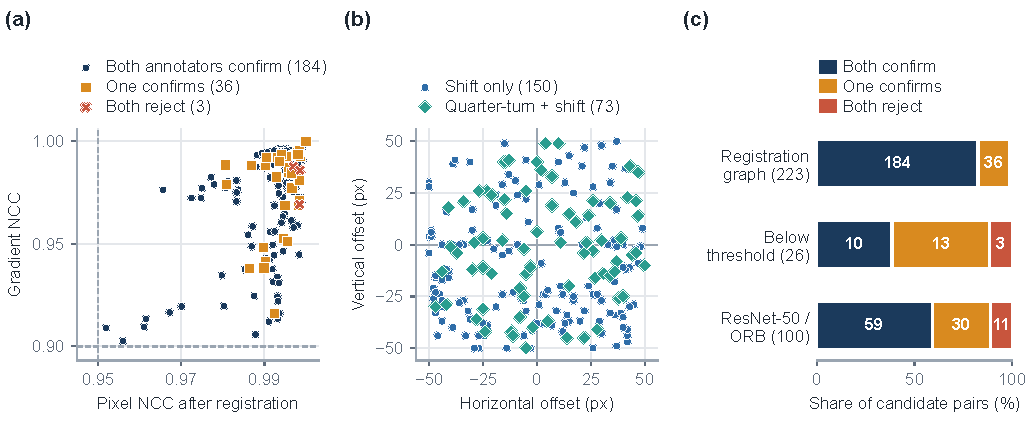
\includegraphics[width=\textwidth]{figures/figB_duplicates.pdf}
\caption{Evidence on the 223 registration edges in NEU-DET. (a) Pixel and gradient correlation after alignment, coloured by the verdict of two independent annotators; dashed lines are the acceptance thresholds. (b) Offset between the two images of each pair; a third of the pairs also differ by a rotation of $90^{\circ}$, $180^{\circ}$ or $270^{\circ}$. (c) Verdicts for the graph edges and for two sets of candidates outside the graph: many pairs outside the graph are also judged to overlap.}
\label{fig:dup_evidence}
\end{figure*}

\begin{table}[htbp]
\centering
\footnotesize
\setlength{\tabcolsep}{2.5pt}
\caption{Sensitivity of near-duplicate graph topology and naive cross-split leakage across coarse ($\tau_{\text{coarse}}$) and native $200\times 200$ thresholds ($\text{NCC}_{\text{pix}}, \text{NCC}_{\text{grad}}$) on NEU-DET ($N=1,797$, overlap $\ge 0.60$).}
\label{tab:threshold_sensitivity}
\begin{tabularx}{\textwidth}{>{\raggedright\arraybackslash}X r r r r r r r}
\toprule
\textbf{Threshold Regime} & $\tau_{\text{c}}$ & $\text{NCC}_{\text{pix}}$ & $\text{NCC}_{\text{grad}}$ & \textbf{Edges} & \textbf{Imgs} & \textbf{Comps} & \textbf{Cross (Tr--Te)} \\
\midrule
Benchmark Graph ($+$band) & 0.80 & 0.95 & 0.90 & \textbf{223} & \textbf{351} & \textbf{147} & \textbf{74 (32)} \\
Primary Coarse Pass Only & 0.85 & 0.95 & 0.90 & 219 & 343 & 143 & 72 (31) \\
Moderate Coarse Gate & 0.90 & 0.95 & 0.90 & 199 & 321 & 135 & 65 (29) \\
Strict Coarse Gate & 0.95 & 0.95 & 0.90 & 145 & 241 & 106 & 44 (20) \\
\midrule
Strict Native Verification & 0.80 & 0.98 & 0.95 & 184 & 292 & 124 & 57 (22) \\
Ultra-Strict Verification & 0.80 & 0.99 & 0.98 & 134 & 219 & 93 & 46 (18) \\
\bottomrule
\end{tabularx}
\end{table}

\subsection{Training Protocol and Hardware}
All detectors are trained for 100 epochs with Ultralytics 8.4.189 (pinned in the launch scripts), \texttt{imgsz=640} and \texttt{batch=8}; except in the module study (Section~\ref{sec:multiarch_mod10s}), training starts from the official COCO-pretrained weights. The four YOLO detectors use SGD ($\eta_0=0.01$, momentum $0.937$, weight decay $0.0005$) in full precision. \texttt{RT-DETR-L} keeps the Ultralytics default \texttt{optimizer=auto}, which resolved to AdamW with a peak learning rate of $0.001$ on NEU-DET and $0.0007$ on GC10-DET, and trains with mixed precision; its training recipe therefore differs from that of the YOLO detectors, and its scores are compared only across its own seeds. Five of its ten NEU-DET runs (seeds 0--4) were interrupted and resumed from their own last checkpoint; their learning-rate schedules in the logs are identical to those of the uninterrupted runs. Checkpoints are chosen by maximum validation fitness on the isolated validation set and evaluated once on the held-out test split at batch size 1 (\texttt{amp=False}).
The experiments comprise 297 training runs on rented or cloud GPUs and 54 earlier runs on a local workstation. Three early NEU-DET baseline runs that two cloud sessions wrote to at the same time were discarded and retrained from scratch; they are not among the 297.
\begin{itemize}[leftmargin=2em, itemsep=0.1em]
    \item \textbf{Seed study} (100 runs; NVIDIA A100, PyTorch 2.14.1): five detectors (\texttt{YOLO11n}, \texttt{YOLOv8n}, \texttt{YOLO11s}, \texttt{YOLOv8s}, \texttt{RT-DETR-L}) $\times$ ten seeds on the primary grouped split of NEU-DET and on the grouped split of GC10-DET.
    \item \textbf{Split study} (30 runs; RTX 3090, PyTorch 2.12.1): \texttt{YOLO11n} on ten grouped splits of NEU-DET $\times$ three seeds.
    \item \textbf{Leakage study} (127 runs; RTX 3090): ten random splits $\times$ five seeds $\times$ two training conditions, plus 27 runs at intermediate partner doses.
    \item \textbf{Module study} (40 runs): four model variants $\times$ ten seeds; seeds 0--4 on the RTX 3090 and 5--9 on the A100, with comparisons paired within seed and machine.
    \item \textbf{Pilot runs} (54 runs; local RTX 4060 laptop GPU, PyTorch 2.7.1): a three-seed comparison of a pilot grouped split with one random split, and a single-split version of the leakage study. They are reported only where stated. The same machine, idle, is used for latency.
\end{itemize}
Across the 297 cloud runs, three GPU environments were used: two Google Colab \texttt{A100-SXM4-80GB} sessions (120 runs total under PyTorch 2.14.1: Colab A with 63 runs [30 \texttt{GC10-CoilGrouped}, 33 \texttt{NEU-Grouped}] and Colab B with 57 runs [20 \texttt{GC10-CoilGrouped}, 17 \texttt{NEU-Grouped}, and 20 \texttt{e7\_modules}]) and one rented RTX 3090 server (177 runs under PyTorch 2.12.1: 127 counterfactual runs, 30 \texttt{e2\_g00}--\texttt{e2\_g09} split runs, and 20 \texttt{e7\_modules} runs). All runs within the same machine used identical software stacks, and A100 baseline runs are comparable across sessions.

Because up to five jobs ran concurrently on the shared GPUs, training time and inference speed from those runs are not used; latency is measured only on a dedicated idle machine (Table~\ref{tab:latency}). \todo{Module study: the four YAML-built variants must be rerun after confirming in the training log that the pretrained weights were actually used (``Transferred \ldots items from pretrained weights''). With the current launcher the weights loaded into the model object are discarded when training starts, so the present runs are very likely trained from random initialisation; this, and not a difference in the number of transferred tensors, would explain the 3.8~pp gap to the standard checkpoint. Describe the corrected procedure here.}

\section{Results}\label{sec:bench_results}

\subsection{How much do scores move when the model does not change?}

\paragraph{Seed.} We trained five detectors ten times each on a fixed split of each dataset, changing only the random seed (Table~\ref{tab:bench_results}, Figure~\ref{fig:seed_noise}a). The standard deviation of test mAP@0.5 over seeds, $\sigma_{\text{seed}}$, is 0.78--1.28~pp on NEU-DET and 1.44--1.98~pp on GC10-DET. Individual classes are much less stable than the mean: for rolled-in scale and crazing the seed standard deviation of class AP reaches 3--4~pp (Figure~\ref{fig:seed_noise}b, Table~\ref{tab:per_class}).

These numbers give the yardstick used in the rest of the paper. If a baseline and a proposed model are each trained once, the difference of their scores has standard deviation $\sqrt{2}\,\sigma_{\text{seed}}$ even when the two models are equally good. The smallest difference that can be distinguished from zero at the 95\% level is therefore
\begin{equation}
\Delta_{\min}=1.96\,\sqrt{2}\,\sigma_{\text{seed}} ,
\label{eq:ruler}
\end{equation}
which is 2.2--3.5~pp on NEU-DET and 4.0--5.5~pp on GC10-DET across the five detectors (2.3--3.5~pp and 4.0--5.2~pp for the four YOLO detectors alone, which share one training recipe). A single-run gain below $\Delta_{\min}$ is compatible with no improvement at all.

\paragraph{Split.} We then trained one detector on ten different registration-grouped splits of NEU-DET, three seeds each (Table~\ref{tab:e2_anova}, Figure~\ref{fig:seed_noise}c). Split means range from 71.0\% to 79.9\%. A one-way random-effects analysis attributes 83\% of the variance of test mAP@0.5 to the split ($\hat{\sigma}_{\text{split}}=2.61$~pp) and 17\% to the seed ($\hat{\sigma}_{\text{seed}}=1.19$~pp; $F(9,20)=15.5$, $p<10^{-6}$).

What this implies depends on the comparison. Within one paper, baseline and proposed model normally share a split, so the split effect largely cancels and Eq.~\eqref{eq:ruler} applies. Across papers it does not cancel: two scores obtained on different, undisclosed splits differ by chance with standard deviation $\sqrt{2(\hat{\sigma}_{\text{split}}^{2}+\hat{\sigma}_{\text{seed}}^{2})}$, and the 95\% threshold becomes 7.9~pp. Copying a baseline number from another paper, which the audit could not rule out for most evaluations (\texttt{F14}), puts a comparison in this second regime. \todo{Whether a gain measured on one split carries over to another (a model-by-split interaction) is not measured here; add the 60-run experiment or state this as a limitation.}

\paragraph{Validation versus test.} Validation mAP@0.5 exceeds test mAP@0.5 by 0.9--2.9~pp for nine of the ten detector--dataset combinations (Table~\ref{tab:bench_results}), which is what selecting the checkpoint on the validation set would produce. A paper that reports the validation score of its selected checkpoint as its result therefore overstates performance by an amount similar to a typical claimed gain; only 5.5\% of evaluations document that they did not.

\begin{figure*}[t]
\centering
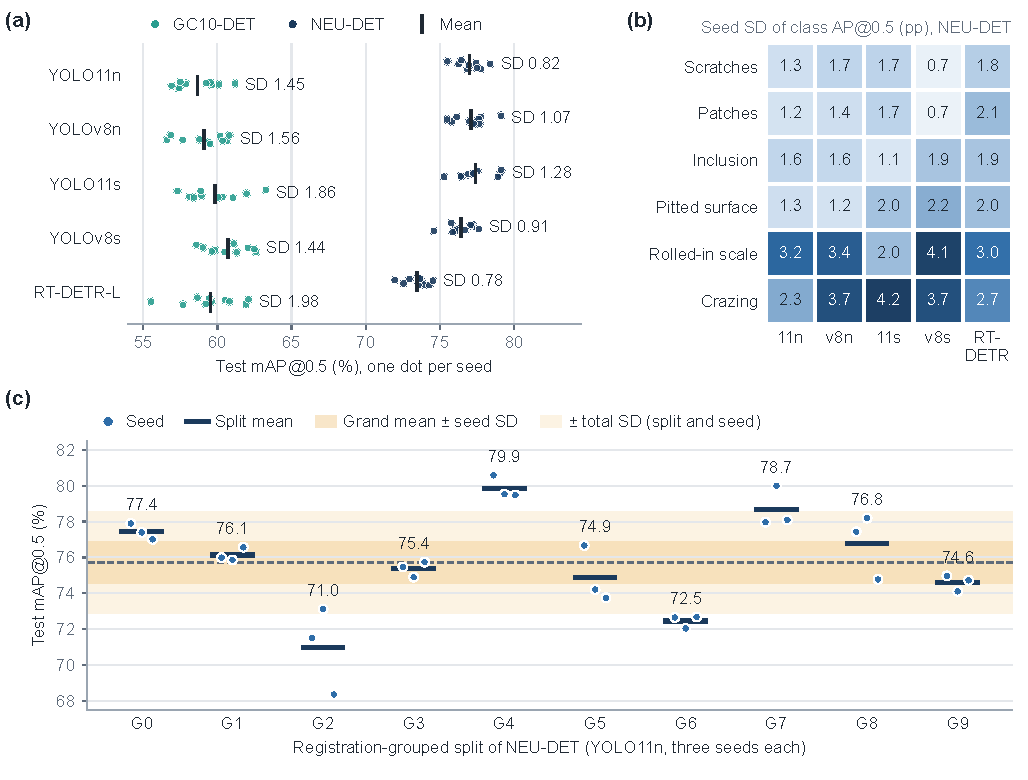
\includegraphics[width=\textwidth]{figures/figC_noise.pdf}
\caption{Variation in test score when the model is unchanged. (a) Ten seeds for each of five detectors on NEU-DET and GC10-DET; SD is the standard deviation over seeds (\texttt{RT-DETR-L} uses its default AdamW recipe, the YOLO detectors SGD). (b) Seed standard deviation of per-class AP@0.5 on NEU-DET. (c) Ten registration-grouped splits of NEU-DET with three seeds each; the bands show the grand mean $\pm$ the seed standard deviation and $\pm$ the total standard deviation.}
\label{fig:seed_noise}
\end{figure*}

\begin{figure*}[t]
\centering
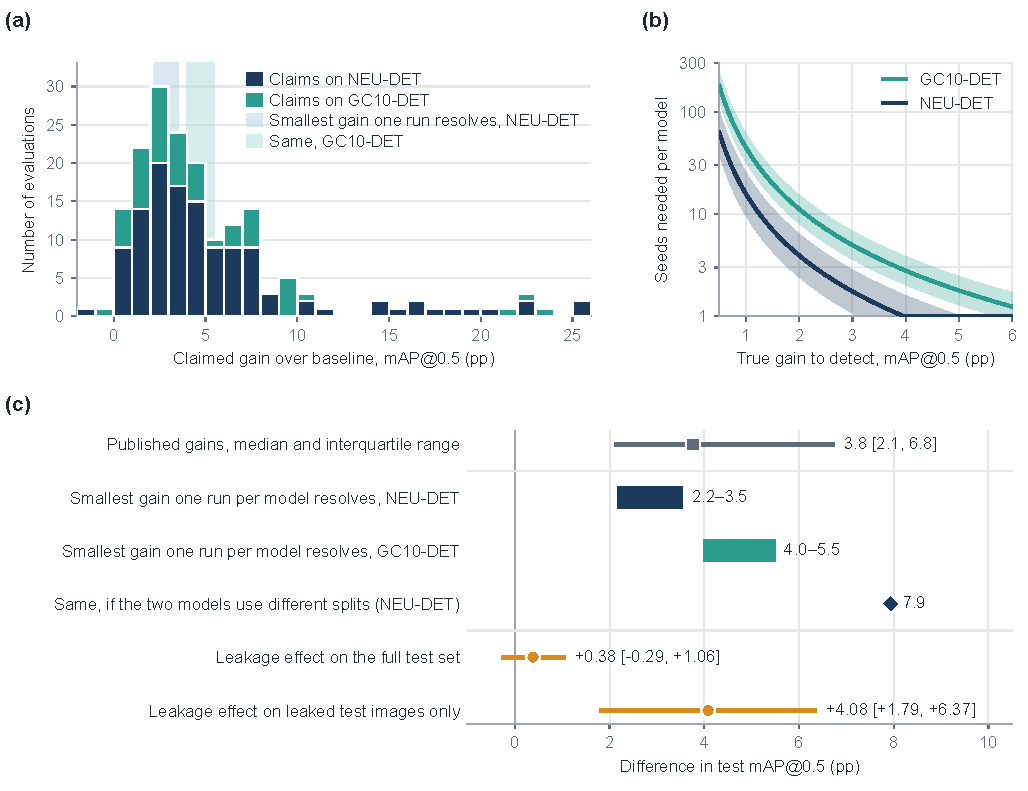
\includegraphics[width=\textwidth]{figures/figD_ruler.pdf}
\caption{Published gains against what a single run can resolve. (a) Gains over baseline extracted from the audited papers (\todo{regenerate from the cleaned table}), with the range of $\Delta_{\min}$ (Eq.~\ref{eq:ruler}) over five detectors for each dataset. (b) Number of seeds per model needed to detect a true gain with 80\% power at the 5\% level; bands span the five detectors. (c) All quantities of this study on one axis: published gains, the single-run resolution limits, and the effect of near-duplicate leakage on the full test set and on the leaked test images alone (95\% confidence intervals over ten paired splits).}
\label{fig:claims_vs_noise}
\end{figure*}

\begin{table}[htbp]
\centering
\footnotesize
\setlength{\tabcolsep}{2.5pt}
\caption{Multi-architecture 10-seed baseline benchmark (100 runs) on registration-grouped \textbf{NEU-Grouped} ($N=1,797$, 0 cross-split edges) and filename-group-disjoint \textbf{GC10-CoilGrouped} ($N=2,291$ across 467 coils, 0 cross-split coil edges), plus the local 3-seed \textbf{NEU-Pilot} vs.\ \textbf{NEU-Random} diagnostic anchor. YOLO detectors use SGD in full precision; \texttt{RT-DETR-L} uses the Ultralytics default (AdamW, mixed precision).}
\label{tab:bench_results}
\begin{tabular*}{\textwidth}{@{\extracolsep{\fill}} l r r r r r}
\toprule
\textbf{Dataset / Detector (Seeds)} & \textbf{Val@0.5} & \textbf{Test@0.5} & \textbf{Rng} & \textbf{Test@50:95} & \textbf{Val$-$Test} \\
\midrule
\multicolumn{6}{l}{\textit{\textbf{NEU-Grouped} ($N=1,797$, zero cross-split edges, 5 detectors $\times$ 10 seeds = 50 runs)}} \\
\texttt{YOLO11n} ($s_0$--$s_9$) & 78.77 $\pm$ 0.98 & 77.01 $\pm$ 0.82 & 2.89 & 44.82 $\pm$ 0.66 & +1.75 $\pm$ 1.57 \\
\texttt{YOLOv8n} ($s_0$--$s_9$) & 78.28 $\pm$ 0.59 & 77.11 $\pm$ 1.07 & 3.65 & 43.76 $\pm$ 0.58 & +1.17 $\pm$ 1.14 \\
\texttt{YOLO11s} ($s_0$--$s_9$) & 79.56 $\pm$ 1.08 & 77.42 $\pm$ 1.28 & \textbf{3.87} & 44.31 $\pm$ 0.64 & +2.14 $\pm$ 1.35 \\
\texttt{YOLOv8s} ($s_0$--$s_9$) & 77.34 $\pm$ 0.89 & 76.42 $\pm$ 0.91 & 3.03 & 43.12 $\pm$ 0.93 & +0.92 $\pm$ 1.36 \\
\texttt{RT-DETR-L} ($s_0$--$s_9$) & 76.41 $\pm$ 1.47 & 73.47 $\pm$ 0.78 & 2.58 & 42.49 $\pm$ 0.69 & +2.94 $\pm$ 1.50 \\
\midrule
\multicolumn{6}{l}{\textit{\textbf{GC10-CoilGrouped} ($N=2,291$, zero cross-coil edges, 5 detectors $\times$ 10 seeds = 50 runs)}} \\
\texttt{YOLO11n} ($s_0$--$s_9$) & 61.10 $\pm$ 1.88 & 58.67 $\pm$ 1.45 & 4.27 & 30.57 $\pm$ 0.85 & +2.43 $\pm$ 2.04 \\
\texttt{YOLOv8n} ($s_0$--$s_9$) & 60.41 $\pm$ 1.64 & 59.08 $\pm$ 1.56 & 4.20 & 30.33 $\pm$ 1.23 & +1.32 $\pm$ 2.67 \\
\texttt{YOLO11s} ($s_0$--$s_9$) & 62.73 $\pm$ 0.85 & 59.83 $\pm$ 1.86 & 5.96 & 30.74 $\pm$ 1.10 & +2.90 $\pm$ 1.46 \\
\texttt{YOLOv8s} ($s_0$--$s_9$) & 60.59 $\pm$ 1.66 & 60.72 $\pm$ 1.44 & 4.02 & 31.07 $\pm$ 1.25 & $-$0.12 $\pm$ 1.59 \\
\texttt{RT-DETR-L} ($s_0$--$s_9$) & 61.87 $\pm$ 2.10 & 59.55 $\pm$ 1.98 & \textbf{6.57} & 29.58 $\pm$ 1.85 & +2.33 $\pm$ 1.85 \\
\midrule
\multicolumn{6}{l}{\textit{Local RTX 4060 Diagnostic Anchor (\texttt{YOLO11n}, $s_0$--$s_2$, 6 runs)}} \\
\textbf{NEU-Pilot} (0 edges) & 76.72 $\pm$ 0.42 & 75.83 $\pm$ 1.53 & 2.92 & 43.16 $\pm$ 0.84 & +0.89 $\pm$ 1.46 \\
\textbf{NEU-Random} (74 edges) & 81.97 $\pm$ 0.98 & 74.72 $\pm$ 0.40 & 0.77 & 43.61 $\pm$ 0.68 & +7.25 $\pm$ 0.88 \\
\bottomrule
\end{tabular*}
\end{table}

\begin{table}[htbp]
\centering
\footnotesize
\setlength{\tabcolsep}{2.5pt}
\caption{Variance decomposition across $G=10$ registration-grouped splits ($G_0$--$G_9$; $G_0 = \text{\textbf{NEU-Grouped}}$) $\times$ $S=3$ seeds = 30 \texttt{YOLO11n} runs on RTX 3090.}
\label{tab:e2_anova}
\begin{tabularx}{\textwidth}{l r r r r | >{\raggedright\arraybackslash}X r r}
\toprule
\textbf{Split} & \textbf{Test50} & \textbf{SD} & \textbf{Val50} & \textbf{50:95} & \textbf{ANOVA Component} & \textbf{Test@0.5} & \textbf{Test@50:95} \\
\midrule
$G_0$* & 77.43 & 0.44 & 79.16 & 45.40 & Grand Mean $\pm$ SD & 75.72 $\pm$ 2.78 & 43.68 $\pm$ 2.41 \\
$G_1$ & 76.14 & 0.38 & 77.25 & 44.31 & Split Means Range & 70.99--79.87 & 39.73--46.68 \\
$G_2$ & \textbf{70.99} & 2.42 & 74.85 & 39.73 & Split Span $\Delta_{\max-\min}$ & \textbf{8.87 pp} & \textbf{6.95 pp} \\
$G_3$ & 75.37 & 0.43 & 78.20 & 44.23 & $\hat{\sigma}_{\text{split}}$ ($\hat{\sigma}^2_{\text{split}}$) & \textbf{2.61 pp} (6.79) & \textbf{2.23 pp} (4.98) \\
$G_4$ & \textbf{79.87} & 0.63 & 77.29 & 46.68 & $\hat{\sigma}_{\text{seed}}$ ($\hat{\sigma}^2_{\text{seed}}$) & 1.19 pp (1.41) & 1.07 pp (1.15) \\
$G_5$ & 74.88 & 1.57 & 78.99 & 41.32 & \textbf{\% Var: Split / Seed} & \textbf{82.8\% / 17.1\%} & \textbf{81.2\% / 18.8\%} \\
$G_6$ & 72.46 & 0.36 & 81.10 & 41.93 & $F(9,20)$ & 15.50 & 13.96 \\
$G_7$ & 78.68 & 1.13 & 75.84 & 45.80 & $p$-value & $3.45\times 10^{-7}$ & $8.21\times 10^{-7}$ \\
$G_8$ & 76.80 & 1.79 & 81.04 & 45.13 & Val mAP@0.5 \% Var & \multicolumn{2}{r}{\textbf{86.4\% Split / 13.6\% Seed}} \\
$G_9$ & 74.60 & 0.44 & 79.21 & 42.31 & Val mAP@0.5 Range & \multicolumn{2}{r}{74.85--81.10 (Span 6.26 pp)} \\
\bottomrule
\end{tabularx}
\end{table}

\begin{table}[htbp]
\centering
\footnotesize
\setlength{\tabcolsep}{3pt}
\caption{Per-category held-out test $\text{AP@0.5}$ (\%) dispersion across 10 seeds on \textbf{NEU-Grouped} (A100), comparing \texttt{YOLO11n} spread and peak 10-seed ranges across all five detectors.}
\label{tab:per_class}
\begin{tabularx}{\textwidth}{>{\raggedright\arraybackslash}X r r r r l}
\toprule
\textbf{Defect Category} & \textbf{YOLO11n Mean$\pm$SD} & \textbf{Min--Max (\%)} & \textbf{Rng} & \textbf{Peak Rng} & \textbf{Worst Arch.} \\
\midrule
\textbf{Crazing} & 39.58 $\pm$ 2.27 & 36.70--42.61 & 5.91 & \textbf{12.83 pp} & \texttt{YOLO11s} \\
\textbf{Inclusion} & 84.28 $\pm$ 1.63 & 82.50--86.92 & 4.42 & 6.75 pp & \texttt{RT-DETR-L} \\
\textbf{Patches} & 94.80 $\pm$ 1.21 & 92.93--96.37 & 3.44 & 7.19 pp & \texttt{RT-DETR-L} \\
\textbf{Pitted Surface} & 80.05 $\pm$ 1.35 & 78.42--82.64 & 4.22 & 6.74 pp & \texttt{YOLOv8s} \\
\textbf{Rolled-in Scale} & 68.93 $\pm$ 3.17 & 63.00--73.32 & \textbf{10.31} & \textbf{11.74 pp} & \texttt{YOLOv8s} \\
\textbf{Scratches} & 94.43 $\pm$ 1.32 & 91.76--95.90 & 4.13 & 6.73 pp & \texttt{YOLO11s} \\
\midrule
\textbf{Macro Mean} & 77.01 $\pm$ 0.82 & 75.51--78.40 & \textbf{2.89} & \textbf{3.87 pp} & \texttt{YOLO11s} \\
\bottomrule
\end{tabularx}
\end{table}

\subsection{How much does near-duplicate leakage add?}\label{sec:counterfactual}\label{sec:leakage_ablation}

\paragraph{Why a naive comparison misleads.} Under a random split of NEU-DET, 74 of the 223 graph edges cross a partition boundary, 32 of them between training and test. The obvious analysis compares the test images that have a training partner (``leaked'' images) with those that do not, and on our first random split the leaked images did score 6.4~pp higher. But leaked images are not a random sample: duplicates are concentrated in some classes (half of all scratches images belong to a component, Figure~\ref{fig:ncc_components}b), and such images may simply be easier. The comparison confounds leakage with difficulty.

\paragraph{Paired design.} We therefore hold the test images fixed and change only the training set. For each of ten random splits, model \textsf{L} is trained on the split as drawn, and model \textsf{C} on the same split with every training partner of a leaked test image replaced by an image of the same class that has no partner in the test set, so that training-set size and class balance are unchanged. Both use the same validation set, from which images linked to training or test images are removed. Each condition is trained with five seeds per split (100 runs). The ten splits contain 300 leaked test images in total (16.7\% of test images; 210 distinct images). Inference treats the split as the unit: seeds are averaged within a split, and intervals and tests use the ten split-level differences. A second series varies the share of partners retained (0, 25, 50, 75, 100\%) on three splits and three seeds.

Because some classes have only one or two leaked images in a given split, macro-averaged mAP on the leaked subset is unstable. We also report AP pooled over classes and instance recall (the share of ground-truth boxes matched at IoU $\ge 0.5$ by a prediction with confidence $\ge 0.25$), and, to connect with inspection practice, miss and escape rates at a fixed number of false positives per image.

\begin{figure*}[t]
\centering
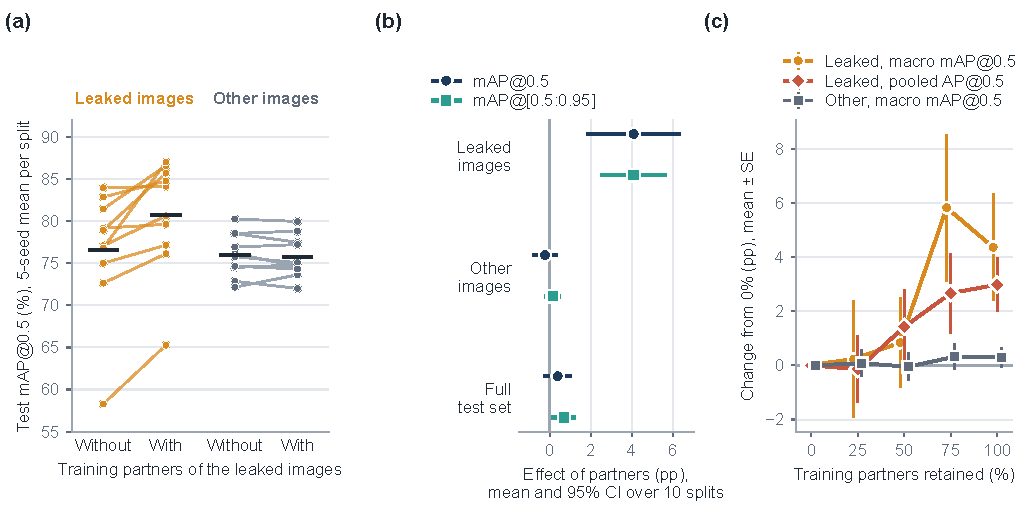
\includegraphics[width=\textwidth]{figures/figE_counterfactual.pdf}
\caption{Effect of near-duplicate training partners, measured on the same test images with and without the partners in training. (a) Split-level scores for leaked and other test images (ten splits; bars are means). (b) Effect by evaluation subset, with 95\% confidence intervals over the ten splits. (c) Change relative to no partners as the share of retained partners grows (three splits $\times$ three seeds, mean $\pm$ standard error).}
\label{fig:leakage_comparison}
\end{figure*}

\begin{figure*}[t]
\centering
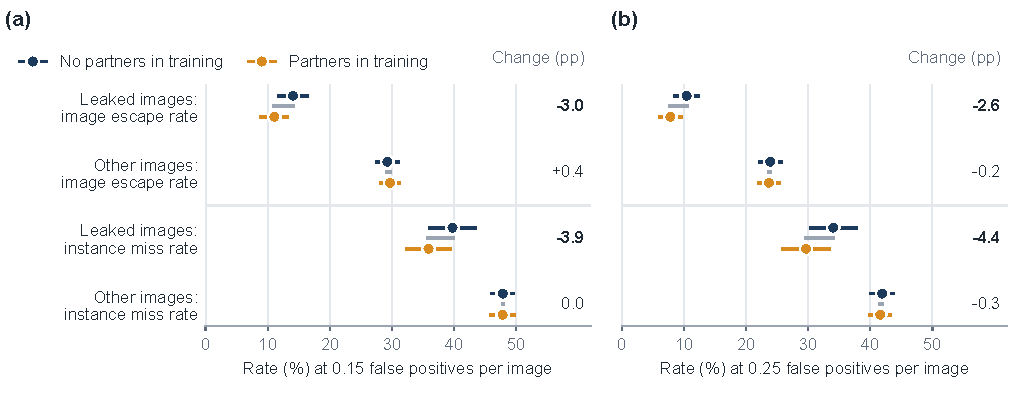
\includegraphics[width=\textwidth]{figures/figF_escape.pdf}
\caption{Miss and escape rates at a fixed false-positive budget, with and without the duplicate partners in training (ten splits, 95\% confidence intervals). The image escape rate is the share of defective images with no correct detection. Bold changes have confidence intervals that exclude zero. Leaked images have much lower rates than other images in both conditions.}
\label{fig:escape}
\end{figure*}

\begin{table}[htbp]
\centering
\footnotesize
\setlength{\tabcolsep}{2.2pt}
\caption{Paired counterfactual results ($K=10$ splits $\times$ $S=5$ seeds $\times$ 2 conditions = 100 runs, RTX 3090; 300 leaked evaluations across 210 unique images). \textsf{L}: trained with the duplicate partners of the leaked test images; \textsf{C}: the same split with those partners replaced. Rows include fixed false-positive operating-point miss and escape rates ($\text{df}=9$ split-level CIs and two-sided Wilcoxon $p$-values).}
\label{tab:counterfactual_ablation}
\begin{tabular*}{\textwidth}{@{\extracolsep{\fill}} l r r r r r r}
\toprule
\textbf{Subset / Metric} & \textbf{\textsf{L}} & \textbf{\textsf{C}} & \textbf{Split $\Delta$} & \textbf{95\% CI} & \textbf{$p_{\text{W}}$} & \textbf{Sign.} \\
\midrule
\multicolumn{7}{l}{\textit{Leaked test images ($T_{\text{leak}}^{(k)}$, 300 image-evals across $K=10$)}} \\
Macro mAP@0.5 (\%) & 80.68 $\pm$ 6.67 & 76.60 $\pm$ 7.32 & \textbf{+4.08 $\pm$ 3.20} & [+1.79, +6.37] & \textbf{0.0020} & \textbf{10/10} \\
Macro mAP@50:95 (\%) & 48.34 $\pm$ 6.23 & 44.26 $\pm$ 6.92 & \textbf{+4.08 $\pm$ 2.25} & [+2.47, +5.69] & \textbf{0.0020} & \textbf{10/10} \\
Pooled Micro-AP@0.5 (\%) & 84.40 $\pm$ 3.83 & 80.85 $\pm$ 4.15 & \textbf{+3.56 $\pm$ 3.18} & [+1.29, +5.83] & \textbf{0.0039} & 9/10 \\
Instance Recall@0.5 (\%) & 78.89 $\pm$ 5.06 & 75.92 $\pm$ 5.25 & \textbf{+2.97 $\pm$ 2.82} & [+0.95, +4.99] & \textbf{0.0078} & 8/10 \\
Macro Recall (\%) & 75.32 $\pm$ 7.10 & 72.08 $\pm$ 7.97 & \textbf{+3.24 $\pm$ 1.99} & [+1.82, +4.66] & \textbf{0.0020} & \textbf{10/10} \\
Macro Precision (\%) & 79.19 $\pm$ 6.08 & 74.05 $\pm$ 6.28 & \textbf{+5.15 $\pm$ 3.66} & [+2.53, +7.77] & \textbf{0.0020} & \textbf{10/10} \\
\midrule
\multicolumn{7}{l}{\textit{Other test images ($T_{\text{clean}}^{(k)}$, negative control)}} \\
Macro mAP@0.5 (\%) & 75.78 $\pm$ 2.48 & 76.01 $\pm$ 2.59 & $-$0.24 $\pm$ 0.86 & [$-$0.85, +0.38] & 0.3223 & 4/10 \\
Pooled Micro-AP@0.5 (\%) & 75.01 $\pm$ 2.22 & 75.25 $\pm$ 2.13 & $-$0.24 $\pm$ 0.75 & [$-$0.78, +0.29] & 0.1934 & 3/10 \\
Instance Recall@0.5 (\%) & 70.57 $\pm$ 3.02 & 70.66 $\pm$ 2.73 & $-$0.09 $\pm$ 1.02 & [$-$0.82, +0.64] & 0.9102 & 5/10 \\
\midrule
\multicolumn{7}{l}{\textit{Overall Held-Out Test Sets ($T_{\text{all}}^{(k)}$, $N=180$ images/split)}} \\
Macro mAP@0.5 (\%) & 76.59 $\pm$ 2.34 & 76.21 $\pm$ 2.27 & +0.38 $\pm$ 0.94 & [$-$0.29, +1.06] & 0.2754 & 7/10 \\
Macro mAP@50:95 (\%) & 45.31 $\pm$ 2.00 & 44.62 $\pm$ 1.96 & \textbf{+0.69 $\pm$ 0.82} & [+0.11, +1.28] & \textbf{0.0137} & 9/10 \\
\midrule
\multicolumn{7}{l}{\textit{Fixed-FP Operating-Point Audit ($0.15$ and $0.25$ FP/img on $T_{\text{all}}^{(k)}$)}} \\
$0.15$ FP: $T_{\text{leak}}$ Inst.\ Miss & 35.89 $\pm$ 5.27 & 39.74 $\pm$ 5.47 & \textbf{$-$3.86 $\pm$ 3.09} & [$-$6.06, $-$1.65] & \textbf{0.0039} & \textbf{10/10}$\downarrow$ \\
$0.15$ FP: $T_{\text{leak}}$ Img.\ Escape & 11.08 $\pm$ 3.25 & 14.07 $\pm$ 3.40 & \textbf{$-$3.00 $\pm$ 2.42} & [$-$4.73, $-$1.27] & \textbf{0.0098} & 9/10$\downarrow$ \\
$0.15$ FP: $T_{\text{clean}}$ Img.\ Escape & 29.67 $\pm$ 2.44 & 29.26 $\pm$ 2.76 & +0.40 $\pm$ 2.02 & [$-$1.04, +1.85] & 0.4258 & 6/10$\uparrow$ \\
$0.25$ FP: $T_{\text{leak}}$ Inst.\ Miss & 29.66 $\pm$ 5.52 & 34.05 $\pm$ 5.36 & \textbf{$-$4.38 $\pm$ 3.03} & [$-$6.55, $-$2.22] & \textbf{0.0020} & \textbf{10/10}$\downarrow$ \\
$0.25$ FP: $T_{\text{leak}}$ Img.\ Escape & 7.82 $\pm$ 2.71 & 10.45 $\pm$ 2.93 & \textbf{$-$2.62 $\pm$ 2.49} & [$-$4.41, $-$0.84] & \textbf{0.0117} & 9/10$\downarrow$ \\
$0.25$ FP: $T_{\text{clean}}$ Img.\ Escape & 23.69 $\pm$ 2.52 & 23.92 $\pm$ 2.74 & $-$0.23 $\pm$ 2.27 & [$-$1.85, +1.39] & 0.7695 & 5/10$\downarrow$ \\
\bottomrule
\end{tabular*}
\end{table}

\paragraph{Leakage is large on the leaked images.} With their partners in training, the leaked test images score $+4.08$~pp higher in mAP@0.5 (95\% CI $[+1.79,+6.37]$; higher in all ten splits) and $+4.08$~pp higher in mAP@[0.5:0.95] ($[+2.47,+5.69]$) than with the partners removed (Table~\ref{tab:counterfactual_ablation}, Figure~\ref{fig:leakage_comparison}a,b). Pooled AP rises by $3.56$~pp ($[+1.29,+5.83]$) and instance recall by $2.97$~pp ($[+0.95,+4.99]$). The other test images are unaffected ($-0.24$~pp, $[-0.85,+0.38]$), which shows that the replacement itself did not change the detector. Per-class effects all point upward but none is estimated precisely enough to exclude zero.

\paragraph{Leakage is small on the benchmark.} The number that matters for a published comparison is the score of the whole test set. Here the effect of leakage is $+0.38$~pp in mAP@0.5 ($[-0.29,+1.06]$), not distinguishable from zero, and $+0.69$~pp in mAP@[0.5:0.95] ($[+0.11,+1.28]$). At the leak rate that random splitting produces on NEU-DET, about one test image in six, leakage is several times smaller than $\Delta_{\min}$ (Figure~\ref{fig:claims_vs_noise}c). It biases every score slightly upward but cannot by itself account for gains of two or three points.

\paragraph{Dose.} Retaining more partners raises the score of the leaked images, though not linearly at low retention: pooled micro-AP is 79.4, 79.2, 80.8, 82.0 and 82.3\% at 0, 25, 50, 75 and 100\% of partners (Figure~\ref{fig:leakage_comparison}c). Across the nine matched (split, seed) series, an ordered trend test confirms a monotonic upward dose response (Page's $L=438.0$, $z=2.20$, two-sided $p=0.028$; one-sided $p=0.014$), with a mean $0 \to 100\%$ linear gain of $+3.51 \pm 3.52\text{ pp}$ ($t(8)=2.99$, $p=0.017$; macro mAP@0.5 Page's $L=444.0$, two-sided $p=0.009$, $0 \to 100\%$ slope $+5.73 \pm 6.43\text{ pp}$, $p=0.028$).

\paragraph{Leaked images are easier to begin with.} Even without any partner in training, the leaked images are detected better than the rest: pooled AP is $5.6$~pp higher ($[+2.7,+8.5]$) and instance recall $5.3$~pp higher ($[+1.0,+9.5]$). In macro mAP the difference averages out over splits ($+0.6$~pp, $[-4.2,+5.4]$) but varies widely from split to split. A naive comparison of leaked and other test images therefore attributes to leakage a difference that is partly, and in some splits mostly, a difference in difficulty.

\paragraph{At a fixed false-positive budget.} With the confidence threshold set to give 0.15 false positives per image on the test set, the share of leaked defective images that receive no correct detection falls from 14.1\% to 11.1\% when the partners are in training ($-3.0$~pp, $[-4.7,-1.3]$), and the instance miss rate from 39.7\% to 35.9\%; at 0.25 false positives per image the image escape rate falls from 10.5\% to 7.8\% (Figure~\ref{fig:escape}, Table~\ref{tab:counterfactual_ablation}). Rates on the other images do not change. Note that the escape rate of the other images, about 29\% and 24\% at the two budgets, is twice that of the leaked images in \emph{both} conditions; that gap reflects which images are leaked, not the effect of leakage. These 0.15 and 0.25~FP/img thresholds are chosen purely as illustrative low-false-alarm operating points rather than empirical production-line settings.


\subsection{Do common modules survive a matched re-test?}\label{sec:multiarch_mod10s}
\todo{This subsection must be rewritten after the rerun. Intended design: three modules that papers commonly add to a YOLO baseline, CBAM \citep{woo2018cbam}, EMA \citep{ouyang2023ema} and BiFPN \citep{tan2020efficientdet}, are each compared with the unmodified model over ten paired seeds on the same split, with the same pretrained weights verified in the training log. Report for each module the paired mean difference with its 95\% confidence interval, and compare it with $\Delta_{\min}$. Then report how often two single runs, one per model, would differ by 2~pp or more by chance. If the confidence interval spans roughly $\pm1$~pp, write ``no gain larger than about 1~pp'' rather than ``no effect''. The values of the current runs are withheld from Table~\ref{tab:v6_multiarch_e7} until the weights issue is resolved (they remain in \texttt{results/cloud\_297\_comprehensive\_stats.json}).}

\begin{table}[htbp]
\centering
\footnotesize
\setlength{\tabcolsep}{1.2pt}
\caption{\todo{Pending rerun with verified pretrained weights.} Module re-test (40 runs of \texttt{YOLO11n} on \textbf{NEU-Grouped}) under pre-fix YAML loading (discarded weights; pending 493-tensor COCO rerun, $s_0$--$s_4$ RTX 3090; $s_5$--$s_9$ A100; paired within matched seed and platform).}
\label{tab:v6_multiarch_e7}
\begin{tabular*}{\textwidth}{@{\extracolsep{\fill}} l r r r c r l}
\toprule
\textbf{Model Variant} & \textbf{Val@0.5} & \textbf{Test@0.5} & \textbf{50:95} & \textbf{Paired $\Delta$50 [CI]} & \textbf{$p_{\text{W}}$} & \textbf{Cherry-Pick*} \\
\midrule
% Values from the pre-fix runs (training started from random initialisation, args.yaml pretrained=false)
% are withheld until the rerun with verified COCO weights; see results/cloud_297_comprehensive_stats.json:e7_modules.
\texttt{YOLO11n-base} & \multicolumn{6}{c}{\todo{rerun pending}} \\
\texttt{+CBAM} & \multicolumn{6}{c}{\todo{rerun pending}} \\
\texttt{+EMA} & \multicolumn{6}{c}{\todo{rerun pending}} \\
\texttt{+BiFPN} & \multicolumn{6}{c}{\todo{rerun pending}} \\
\bottomrule
\end{tabular*}
\par\vspace{0.3em}\noindent{\footnotesize *Best variant test seed minus lowest baseline test seed within platform (RTX 3090 / A100); parenthetical (\texttt{v}) values use best validation $\text{mAP@0.5}$.}
\end{table}

\subsection{Stage-Wise Inference Latency Accounting}
To demonstrate transparent compliance with dimension \texttt{F15}, Table~\ref{tab:latency} separates stage-wise timing measured during isolated single-job execution on an idle RTX 4060 Laptop GPU (batch size 1, FP32 \texttt{amp=False}, $640\times 640$, test $N=180$, three seeds). Reporting preprocessing ($0.42\text{ ms}$) and NMS ($0.78\text{ ms}$, $10.6\%$ of end-to-end runtime) separately from backbone forward pass ($6.17\text{ ms}$) avoids conflating pure forward throughput ($162.1\text{ FPS}$) with deployed end-to-end line speed ($135.5\text{ FPS}$).

\begin{table}[htbp]
\centering
\footnotesize
\setlength{\tabcolsep}{5pt}
\caption{Isolated single-job stage-wise inference latency accounting for \texttt{YOLO11n} on an idle NVIDIA RTX 4060 Laptop GPU (batch size 1, FP32, $640\times 640$, $N=180$, 3 seeds).}
\label{tab:latency}
\begin{tabular}{l r r r}
\toprule
\textbf{Pipeline Stage} & \textbf{Latency (ms)} & \textbf{SD (ms)} & \textbf{Throughput (FPS)} \\
\midrule
Preprocessing (Letterbox \& Normalization) & 0.42 & $\pm$ 0.01 & 2,381.0 \\
Model Forward Inference & 6.17 & $\pm$ 0.07 & 162.1 \\
Postprocessing (NMS, $\text{IoU}=0.70$) & 0.78 & $\pm$ 0.03 & 1,282.1 \\
\midrule
\textbf{Total End-to-End Latency} & \textbf{7.38} & $\pm$ \textbf{0.09} & \textbf{135.5} \\
\bottomrule
\end{tabular}
\end{table}

\section{Discussion}\label{sec:discussion}

\subsection{What the four answers add up to}
The audit shows that a reader cannot check a published gain: the split is never released, the seed almost never, and nine evaluations in ten give a single number. The experiments show what that single number is worth. On a shared split, one run per model resolves differences of 2.2--3.5~pp on NEU-DET and 4.0--5.5~pp on GC10-DET; on different splits, about 8~pp. \todo{Give the share of published gains below these thresholds.} Near-duplicate leakage, the explanation most often suspected, turns out to be a smaller effect at the level of the benchmark: under random splitting it shifts the full-test score by less than one point. It still matters. It biases every reported number upward, it is concentrated in a few classes, and on the affected images it changes detection rates at a fixed false-positive budget by several points, which is the quantity an inspection line cares about. But the main reason single-run gains on these benchmarks cannot be read is ordinary run-to-run and split-to-split variation that is not reported.

This does not mean that the published gains are wrong. A gain below $\Delta_{\min}$ may be real; a single run simply cannot show it. \todo{Add the module result here once it is final.}

\subsection{How many seeds does a claim need?}
The resolution limit can be turned around into a planning rule. To detect a true gain $\delta$ with 80\% power at the 5\% level, each model needs approximately
\begin{equation}
n \approx \frac{2\,(1.96+0.84)^{2}\,\sigma_{\text{seed}}^{2}}{\delta^{2}} \approx 15.7\,\frac{\sigma_{\text{seed}}^{2}}{\delta^{2}}
\end{equation}
seeds (Figure~\ref{fig:claims_vs_noise}b). With the standard deviations measured here, showing a 2~pp gain takes 3 to 7 seeds per model on NEU-DET and 9 to 16 on GC10-DET; showing a 1~pp gain takes 10 to 26 on NEU-DET and more than 30 on GC10-DET. In our setup a 100-epoch run of \texttt{YOLO11n} on NEU-DET took about one hour on a shared RTX 3090 (median 59--61~min; wall-clock time on shared GPUs is indicative only), so the first of these is affordable for any paper.

\subsection{Recommendations}
For authors and reviewers of steel defect detection papers we suggest five minimum requirements, each tied to an audit item.
\begin{enumerate}[leftmargin=2em, itemsep=0.1em]
    \item \textbf{Release the split} as a list of file names (\texttt{F03}). A ratio such as 8:1:1 does not identify a split, and split choice moves scores by several points.
    \item \textbf{Group related images before splitting} (\texttt{F04}): by coil or strip identifier where one exists, otherwise by image registration or feature similarity. State what the grouping can and cannot detect.
    \item \textbf{Select on validation, report on test} (\texttt{F06}--\texttt{F08}), and say so.
    \item \textbf{Retrain the baseline under the same protocol and report several seeds for both models} (\texttt{F12}--\texttt{F14}), with the paired difference and its confidence interval. The rule above gives the number of seeds.
    \item \textbf{Report latency by stage on an idle machine} (\texttt{F15}), separating pre-processing, inference and post-processing.
\end{enumerate}
For an engineer selecting a detector, the practical reading is: treat a single-run difference below about 3~pp on NEU-DET or 5~pp on GC10-DET as a tie, do not compare numbers taken from different papers, and check class-level results for rolled-in scale and crazing over several seeds, since these classes vary most.

\subsection{Limitations}
\begin{enumerate}[leftmargin=2em, itemsep=0.1em]
    \item \textbf{Audit corpus.} Full texts come from the PubMed Central open-access subset indexed by Europe PMC. Articles in subscription journals are not included, and their reporting practice may differ. \todo{Report the cross-database sample here once it has been screened and coded.}
    \item \textbf{Audit coding.} First-pass coding was model-assisted. \todo{State the extent and result of human verification.} The three interpretive items (\texttt{F07}, \texttt{F08}, \texttt{F14}) are the least reliable.
    \item \textbf{Completeness of the duplicate graph.} The registration graph requires at least 60\% overlap and misses pairs that two annotators judge to overlap (Section~\ref{sec:frozen_partition}). The grouped splits remove registration-detected pairs only, and the leakage estimates are lower bounds.
    \item \textbf{Leak rate.} The benchmark-level effect of leakage is measured at the leak rate that random splitting produces on NEU-DET (about 17\% of test images). A dataset with more duplication would show a larger effect.
    \item \textbf{GC10-DET grouping.} Groups on GC10-DET are defined by a field in the file names, which we take to identify a coil or acquisition sequence; this is an assumption. No registration audit was run on GC10-DET. The 2,291-image set excludes three of the 2,294 raw GC10-DET files documented in the curation log: two with no object bounding boxes in their XML annotations (\texttt{img\_02\_4406772100\_00175} and \texttt{img\_06\_3402617700\_00988}) and one containing an unmapped class label \texttt{d} (\texttt{img\_02\_425616500\_00770}).
    \item \textbf{Scope of the experiments.} Five detectors, 100 epochs, one training recipe for the four YOLO detectors and the Ultralytics default recipe (AdamW, mixed precision) for \texttt{RT-DETR-L}. Seed variance may differ for other recipes. NEU-DET images are $200\times200$ crops, so false positives per image and escape rates are not directly comparable with figures from a production line.
    \item \textbf{Split effects on gains.} We measure how much split choice moves a score, not whether it changes the difference between two models.
\end{enumerate}

\section{Conclusion}\label{sec:conclusion}

A gain of two or three points of mAP@0.5 from a single training run, the kind of evidence most steel defect detection papers offer, is within the range that a change of random seed alone produces on NEU-DET and GC10-DET, and well within the range produced by a change of split. Near-duplicate images do leak between training and test data in NEU-DET, and the affected images are detected better as a result, but at the benchmark level this effect is smaller than seed noise. Because papers almost never report seeds, splits or repeated runs, readers cannot tell which published gains would survive. The remedy is cheap: release the split, group related images, and run enough seeds for the size of gain being claimed. The splits, run logs and code released with this paper are intended to make that the default.

\backmatter

\section*{Declarations}

\noindent\textbf{Funding}: The authors declare that no external funding was received for this study.

\vspace{0.4em}
\noindent\textbf{Competing Interests}: The authors have no relevant financial or non-financial interests to disclose.

\vspace{0.4em}
{\emergencystretch=2em
\noindent\textbf{Data Availability}: The public NEU-DET and GC10-DET datasets analyzed in this study are available from their original creators \citep{song2013neu,he2020neu,lv2020gc10}. All derived grouped split manifests (\textbf{NEU-Pilot} [\texttt{372b6745}], \textbf{NEU-Grouped} [\texttt{1a635ccf}], $G_0$--$G_9$, \textbf{GC10-CoilGrouped} [\texttt{ead84d9f}], and counterfactual pairs $K_0$--$K_9$), the 223-edge registration graph, 349-pair human visual annotations, 297-run benchmark logs, and 182-evaluation audit extraction tables are released at \url{https://github.com/bigovennnn/steel-defect-benchmark-audit}.\par}

\vspace{0.4em}
\noindent\textbf{Code Availability}: All Python scripts for Europe PMC PRISMA querying, JATS XML verbatim matching, $\mathrm{SE}(2)$ registration, MIP grouped splitting, counterfactual training, operating-point escape evaluation, and figure reproduction are publicly available at \url{https://github.com/bigovennnn/steel-defect-benchmark-audit}.

\vspace{0.4em}
\noindent\textbf{Author Contributions}: Wenzhuo Liu and Shiling Yu jointly conceived the study, designed the protocol rubric and registration pipeline, independently performed the double-blind visual annotation of 349 image pairs, conducted the experiments and statistical analyses, and wrote and approved the final manuscript.

\vspace{0.4em}
\noindent\textbf{Declaration of Generative AI and AI-Assisted Technologies}: A large language model was used for first-pass screening of titles and abstracts, for first-pass coding of the 17 audit items with supporting quotations, for writing analysis scripts, and for language editing (Section~\ref{sec:lit_method}). \todo{State exactly which outputs were verified by the authors and how; do not claim verification that has not been done.} The authors take full responsibility for the content of the publication.

\bibliography{refs}

\end{document}
